\documentclass[12pt]{article}
\usepackage{titling}
\usepackage{amsmath}
\usepackage{graphicx}
\usepackage{caption}
\usepackage{subcaption}
\usepackage{hyperref}
\usepackage{mathrsfs}
\newcommand{\ts}{\textsuperscript}
\newcommand{\subtitle}[1]{%
  \posttitle{%
    \par\end{center}
    \begin{center}\large#1\end{center}
    \vskip0.5em}%
}



\begin{document}

%

\title{Measures of Cognitive Distance and Diversity.}
\author{Johannes  Castner}		% used by \maketitle

\date \today
\maketitle

\begin{abstract}
This paper explains and demonstrates how a model of human causal learning, {\it Causal Support} (Tenenbaum \& Griffiths, 2001, Griffiths \& Tenenbaum, 2005), can be used to derive an Information theoretic quantity, the Jensen-Shannon Divergence, with which to measure {\it Cognitive Distance}, the degree to which two people differ in their opinions about the workings of the world. It is then shown how this measure is generalized to measure {\it Cognitive Diversity}, the degree of heterogeneity of opinions within a collection of individuals, such as a political party or a research department of a firm or university. These measures are important for theoretical and empirical work on the relationships between Cognitive Diversity and an organization's success in recognizing structure in the universe of interest and in making collective decisions.
\end{abstract}

\newpage

\section{Introduction}
%Here's how I can see your paper:
%A) motivation of big project: aggregation of diverse beliefs. Want to measure relationship of diverse beliefs to performance
%I can't find a good place for the following, but I think that it would make the introduction even stronger:

%\\

An understanding of the conditions for collective wisdom and the mechanisms that enable collectives to become wiser, are at the core of what we might hope to call a science of sustainable development. Most decisions that are relevant to sustainable development, however we may define it, are at least indirectly influenced by human collectives (i.e. committees, congress, corporate boards etc.). One important set of machanisms relates the diversity of individual minds within a collection to the wisdom with which it solves its problems (collective decision and collective action). In economics and political science much has been done to uncover important mechanisms with respect to heterogenous preferences, information asymmetries and even the diversity of received signals (information) when beliefs are homogenous, in market settings and strategic games. However, the situation in which information and goals are the same among members of a collection but beliefs are heterogenous (such as in a team), has to my knowledge not been given much attention and neither have those situations, which are likely to be quite common in our world, where both beliefs and goals, or both beliefs and information-selection are diverse (people endogenously select their sources). Climate change discussions at all scales (from local to global) for example, are likely to draw attendees with highly diverse goals and beliefs, who also are exposed to very different information.\\

Starting with Condorcet's jury theorem, (Marquis de Condorcet, 1785)\footnote{Although since Waldron (1995) there has been widespread argreement among scholars that in \textit{Politics} Aristotle had already espoused a theory of ``The Wisdom of the Multitude'', which implicitly was synonymous with a theory of the social benefits of Diversity, Cammack (2013) convincingly dispelled this interpretation of Aristotle's text and showed that Aristotle, very likely, had something very different in mind.}, there have been various arguments with different degrees of sophistication, that, depending also on the organizational scheme of the collective, many thinkers together will on average come to wiser conclusions than any individual could on her own. In general, in these arguments the implied reason is that the greater the number of people, the greater is the variance in insights (the cognitive heterogeneity and diversity is higher in larger groups, by assumption) and it is this diversity of minds and not the sheer number of people that is believed to lead to better collective decisions\footnote{In the case of Condorcet's jury theorem the argument is simply numerical and has little to do with people's cognition at all.}.  Analogous with the definition of bio-diversity as the amount of genetic information that is available to the system (for greater functional diversity under a greater range of circumstances), an organization's cognitive diversity can be defined as the collective's current available theoretical tool kit and it should thus increase the degree of accuracy with which the collective will judge the workings of the world, under a greater number of contingencies\footnote{Whether and to what degree this is true for any given organization must depend also on the organization's opinion aggregation scheme, just as the benefits of bio-diversity depend on the structure of the food web.}. This, in turn, should improve the collective interaction of the organization with the world; particularly if the world of interest is constantly changing. Models of the world (to be made precise below) that had been inaccurate previously, might have more explanatory power as circumstances change, while those models that once furnished the best explanations might fade in relevance. For a thorough discussion and overview of the literatures on and related to collective wisdom, distributed intelligence/cognition or the wisdom of crowds, see ``Collective Wisdom: Principles and Mechanisms'' (edited by Landemore and Elster, 2012).\\

In much, but not all of this and related work, the number of people in a group of thinkers acts as a proxi for diversity in the absence of a direct measure, which leaves open all questions concerning the differential cognitive diversity in groups with more or less the same fixed number of members. Although diversification of investment in resources and capital has long been standard advise in portfolio theory, not much is known or recommended in terms of the diversification of investment in human resources, with the notable exception of some recent theoretical work by Hong and Page (2004) which has inspired the present work. Additionally, this research direction could give rise to some nuanced and unorthodox policy recommendations for the educational sector. For example, it may result in the advise to expose different students (at all ages and levels) to varying educational opportunities, suited to their own individual needs and desires.\\

Socially constructed measures of diversity (along ethnic, gender and religious dimensions, for example), the definitions of which are highly sensitive to context and interpretation, have become a common public agenda of firms and organizations. This diversity agenda is promoted mostly for ethical and esthetic reasons or as a result of political pressures, while perhaps the most relevant form of diversity, for the success and robustness of collectives, is related to cognition and beliefs. I content that the current lack of a natural measure of cognitive diversity stands in the way of constructing falsifiable theories directly relating the cognitive diversity of a collective to its collective wisdom and that this lack leads to an impasse which helps to explain the current dirth in the theory and empirics of this important subject.  Note however, that, depending on the context, socially constructed measures of diversity might be highly correlated with cognitive diversity, and thus they may serve as more applicable proxies of cognitive diversity than membership size which is often constrained. Thus, a focus on these often more easily apparent forms of diversity might be justifiable not only on ethical or esthetic grounds, but also on grounds of organizational efficacy and robustness, if cognitive diversity can indeed be scientifically shown to have such benefits.  As a requisite for such scientific work, however, adequate and theoretically well-motivated measures of \textit{cognitive distance} (between any two individuals) and \textit{cognitive diversity} (for a collection of individuals) are needed\footnote{If the mechanisms by which cognitive diversity impacts performance and robustness can then be sufficiently isolated and it can be shown that this form of diversity indeed correlates with the other forms, it may be found simpler and more convenient to use more easily visable proxies in actual practice (for example, in human resource departments of firms).}. Thus, this paper concerns itself with such measures. The here advanced cognitive distance metric is the square root of a measure known as the Jensen-Shannon Divergence (henceforth JSD). JSD is an important information theoretic quantity that will here be derived from recent work in cognitive science on how humans uncover causal structure in their universe of concern (Tenenbaum \& Griffiths, 2001, Griffiths \& Tenenbaum, 2005). JSD is then generalized and the square-root of the resulting quantity (known as the $n$-point JSD, or generalized JSD), with the apropriate normalization, is argued to be a meaningful metric of group level cognitive diversity.

\section{Causal Beliefs and Joint Distributions}
%B) This paper: describing causal beliefs and measuring diversity

\begin{figure}
        \centering
        \begin{subfigure}[b]{0.3\textwidth}
                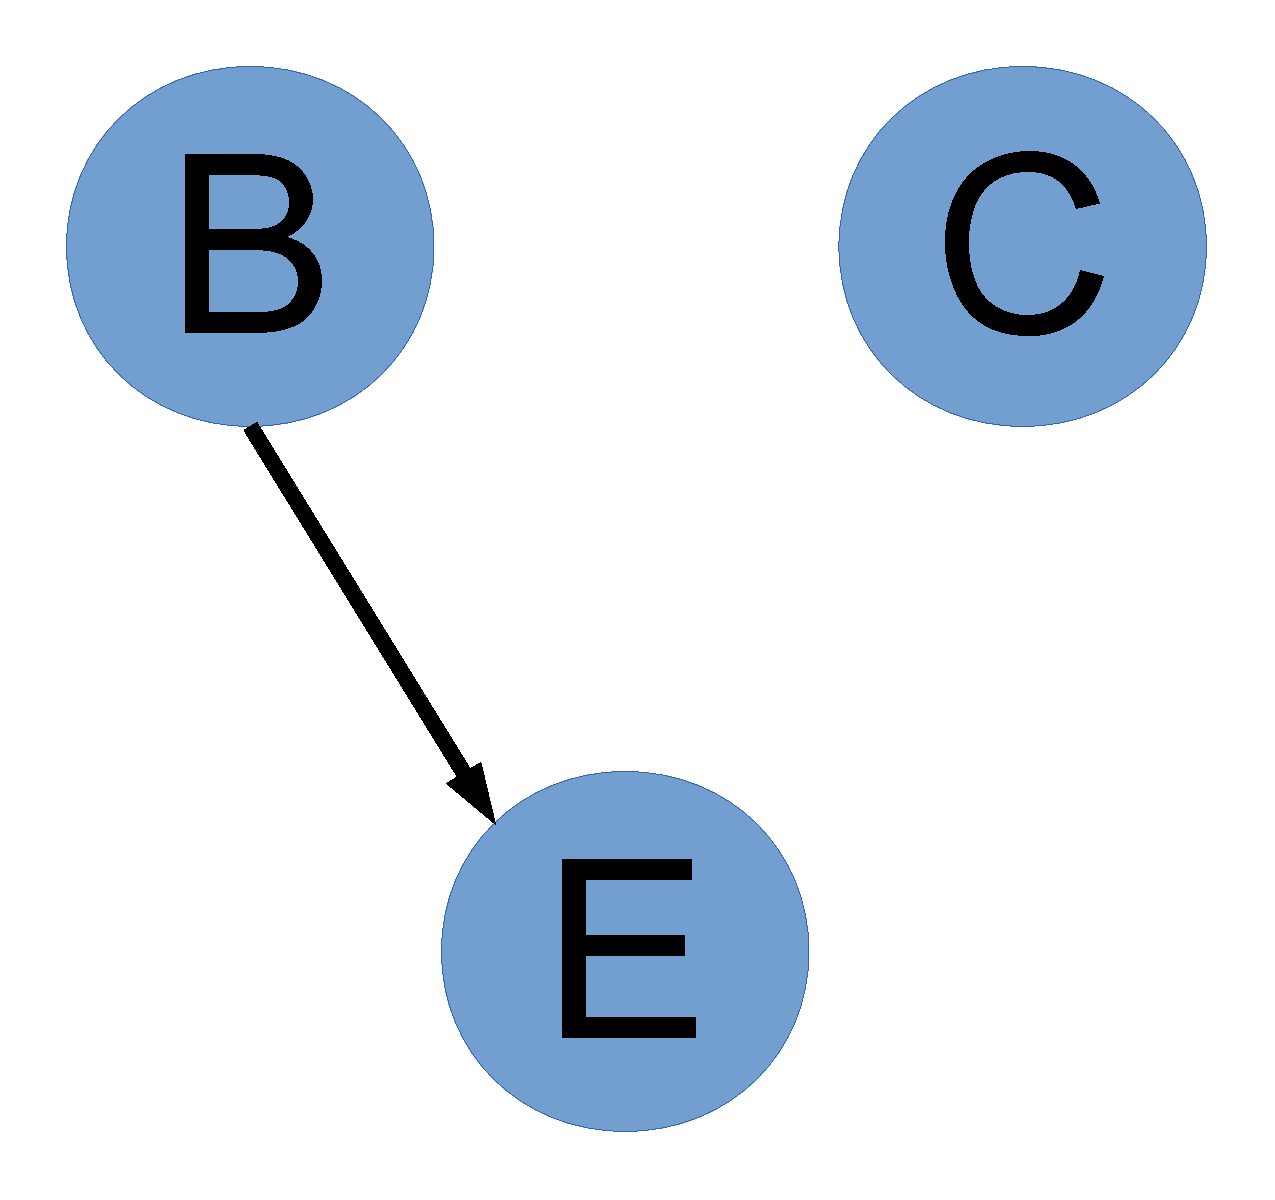
\includegraphics[width=\textwidth]{Graph0.pdf}
                \caption{Graph 0}
                \label{fig:gull}
        \end{subfigure}%
        ~ %add desired spacing between images, e. g. ~, \quad, \qquad etc.
          %(or a blank line to force the subfigure onto a new line)
        \begin{subfigure}[b]{0.3\textwidth}
                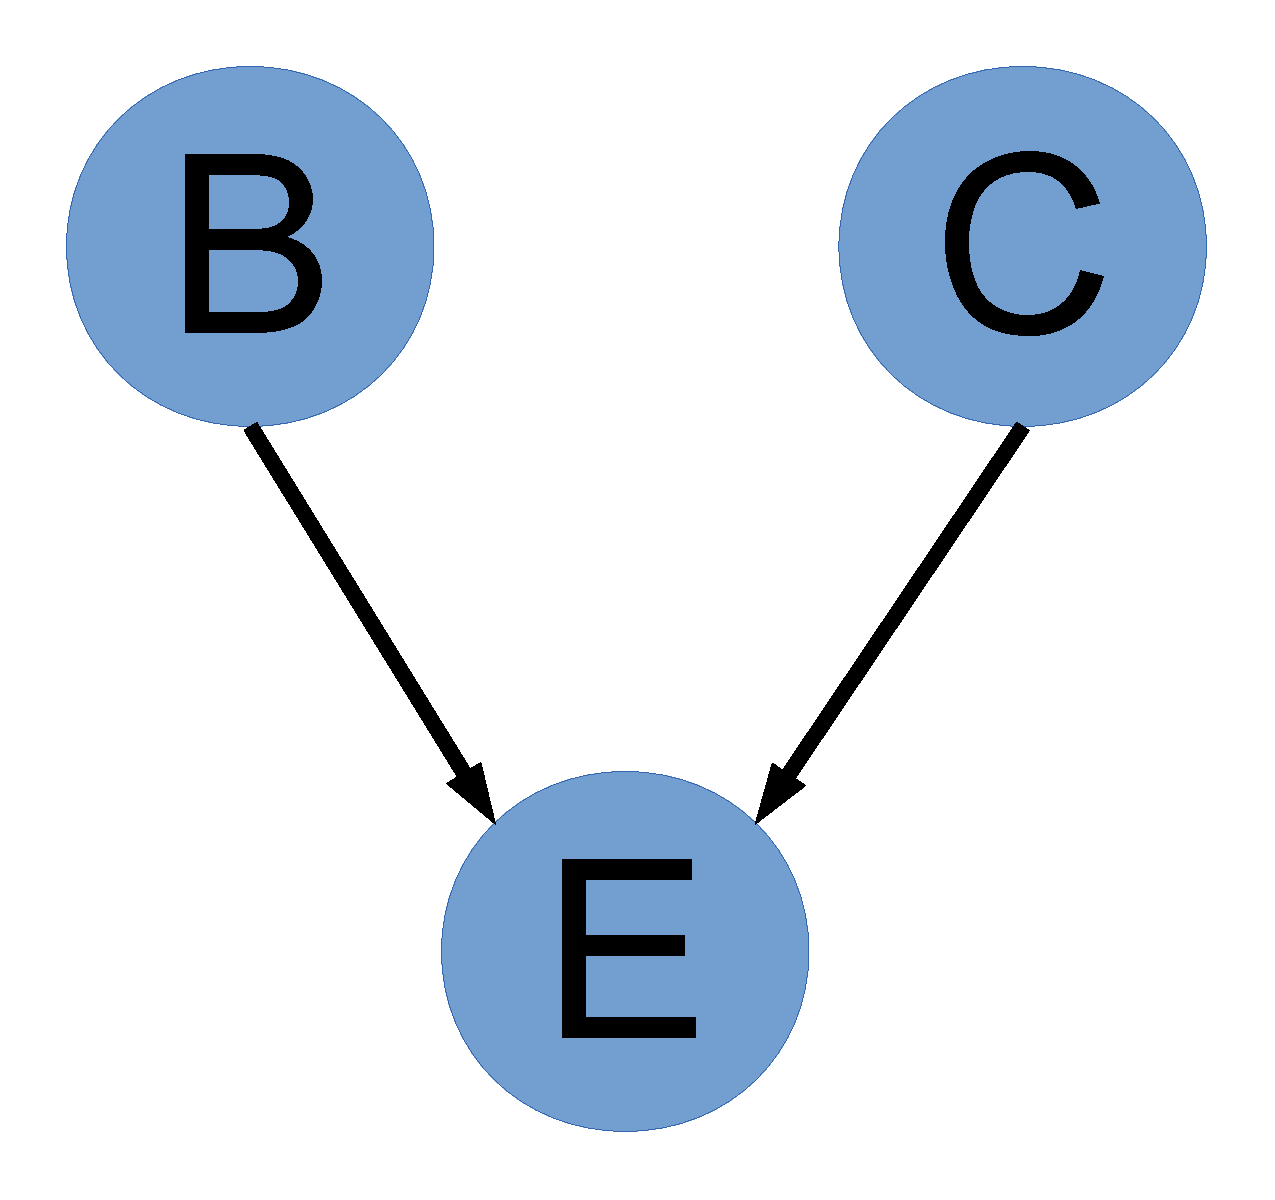
\includegraphics[width=\textwidth]{Graph1.pdf}
                \caption{Graph 1}
                \label{fig:tiger}
        \end{subfigure}
        ~ %add desired spacing between images, e. g. ~, \quad, \qquad etc.
          %(or a blank line to force the subfigure onto a new line)
        \caption{Two examples of Simple Cognitive Maps. Here ``B'' stands for Background Cause and ``C'' stands for Cause of interest (the variable which actor 1 believes has a causal effect on ``E'', but actor 0 does not).}\label{fig:animals}
\end{figure}

Underlying many of the important discussions in business, politics and sustainable development are matters of causality and causal reasoning. Thus, as a preliminary step, this paper restricts itself to the causal domain, although it is acknowledged that other forms of reasoning (ontological, deontic, deontological, etc.) quite often play important roles and must be incorporated to account completely for the diversity of individual reasoning within a collective. Here, ``reasoning'' replaces ``cognition'' to temporarily draw attention to the fact that the measures of cognitive distance and diversity are constructed not from data of cognition per se, as cognition at this scale is unobservable, but from observable reasoning. Either interviews or transcriptions of speeches/debates are used to elicit statements of the form ``CO$_2$ causes Climate Change,''  which are then encoded as directed signed arcs of the graph representing a particular speaker's belief system as depicted in Figure ~\ref{fig:animals}:
$$\text{CO}_2 \xrightarrow{+} \text{Climate-Change}.$$
For macro-economists, for example, the universe of discourse would include variables such as interest rates, unemployement, GDP and inflation, among others. \textit{Cognitive Maps} (henceforth CM), as the resulting signed digraphs are often called (see Figure ~\ref{fig:animals} for two simple examples), can then be coded as \textit{Bayesian Networks} (henceforth BN), which are structural representations of how a person believes that a set of variables is jointly distributed, while maintaining the causal interpretation.
For a detailed account of how beliefs are elicited and cognitive maps are constructed from people's statements see ``Structure of Decision: The Cognitive Maps of Political Elites'' (1976), edited by Robert Axelrod.\\

While the exact calculations in this paper are restricted to arguments of ``linear causation''\footnote{The exact functional relationship as specified by the intuitive Noisy-OR parameterization is sub-linear for multiple causes, to be more precise.}, i.e. unconditional causal effects, making causal effects conditional on the values of various variables is a straight-forward generalization that is exhaustive of all possibilities, as far as causation is concerned\footnote{Any functional probabilistic relationship between any $k$ variables can be specified as part of a Bayesian Network, but such an excercise is not the point of this paper.}. There are two possibly related reasons why linear causal beliefs are of special interest; 1) in human discussions (the data), people tend to express themselves in terms of positive and negative causal relations (Axelrod et. al 1976) and it would be absurd to introduce arbitrary functional relations between variables as part of characterizing people's beliefs and 2) recent theories and empirical results in cognitive science suggest that people are indeed simple in their beliefs of how variables affect each other, which, as shown in Griffiths and Tennenbaum (2005), naturally leads to Pearl's ``Noisy-OR'' parameterization (Pearl, 1988), described in detail below.\\

To show how CMs are encoded as BNs, I closely follow Griffiths, Kemp \& Tenenbaum (2008). For illustrative purposes, two very simple CMs are shown in Figure ~\ref{fig:gull} and Figure ~\ref{fig:tiger}. The universe of discourse is a set of three variables: a background cause $B$, a potential cause of interest, $C$, about the effect of which on $E$ (the effect variable) there is a dispute. The person, let me call him $0$, a representation of whose belief-system (Graph$_0$) is depicted in Figure ~\ref{fig:gull} believes that only $B$ and not $C$ causes $E$, while the person, whom I call $1$, with beliefs represented by Graph$_1$ in Figure ~\ref{fig:tiger}, believes that both $B$ and $C$ exert a causal influence on $E$. For the time being, I'm assuming all believed effects to be positive, but it is later shown how to accomodate negative effects in a principled and straight forward manner. Graph$_0$ is encoded as follows as a Bayesian Network (or simply joint distribution). The joint distribution of any $k$ variables ($k=3$ in this case) can be written as the product of all of its conditionals and its marginals. In the case of Graph$_0$:
%C) In math, define a causal belief structure, and relate it to a probability density function
$$P_0(B, C, E)= P(E | B)*P(B)*P(C)$$
Note that since $B$ is believed to cause $E$, the value of $E$ is believed to depend on the value of $B$ and thus the term $P(E | B)$ is included. However, $E$ is believed to be independent from $C$ and thus $P(E | B, C)$ collapses, while in Graph$_1$ the term would have to be $P(E | B, C)$:
$$P_1(B, C, E)= P(E | B, C)*P(B)*P(C).$$
I assume that all variables are binary (i.e. they can only take on values $0$ and $1$). One could see this assumption as coming from a theory of how people think, where people are theorized to coarse-grain variables as either taking on a high value ($1$) or a low value ($0$), or alternatively the values ($0$, $1$) could be thought of as deviations from some base-line, where $0$ means a decrease and $1$ denotes an increase (with an innocuous assumption that the values of the underlying variables never stay exactly the same).
For a positive causal relation, when $B$ is believed to be the cause of $E$ for example, we have:
$$P(E=1 | B=1) > P(E=1 | B=0),$$
which in the case of Graph$_0$, where there is only one causal variable, can simply be parameterized as:
$$P_0(E=1 | B=b) = \pi_{0, B}b,$$
so that when $b$ equals $0$, the probability of $E$ taking on the value $1$ is believed to be $0$ and when $b$ equals $1$, this is believed to cause $E$ to take on the value $1$ with probability $\pi_{0, B}$. Note that the effect parameters, such as $\pi_{0, B}$, are themselves taken to be drawn from some known distributions and while Griffiths and Tennenbaum assume uniform distributions on the interval $\left[0, 1\right]$, for this paper all calculations have been done using beta distributions as they are more flexible. The beliefs as represented in Graph$_1$, pertaining to $E$s dependence on both $B$ and $C$ ($P_1(E | B, C)$), are slightly more difficult to parameterize. A parameterization that assumes a simple linear dependence on both causes ($P_1(E=1 | B=b, C=c) = \pi_{1, B}b + \pi_{1, C}c$) would introduce a dependence between the two parameters which likely has not explicitly been stated as part of the person's beliefs ($\pi_{1, B} + \pi_{1, C} < 1$), in virtue of preserving the axioms of probability. Note that with more than two causes this becomes even more problematic. Thus, I follow the recommendation in Griffiths, Kemp, \& Tenenbaum (2008) in using Pearl's 1988 Noisy-OR parameterization:

\begin{equation} \label{eq:noisy-or}
P_1(E=1 | B=b, C=c) = 1- (1-\pi_{1, B})^b(1- \pi_{1, C})^c.
\end{equation}

In Equation ~\ref{eq:noisy-or}, we have that if $b$ and $c$ are both equal to $0$, the probability of $E$ taking on the value $1$ is $0$, if only $b$ equals $1$ while $c$ equals $0$, this probability is $\pi_{1, B}$ and if $b$ equals $0$ while $c$ equals $1$ this probability is $\pi_{1, C}$. Lastly, and this is the case for which things change compared to the linear parameterization, when both $b$ and $c$ are equal to $1$, the probability of $E$ taking on tha value $1$ is:

$$P_1(E=1 | B=1, C=1)= \pi_{1, B} + \pi_{1, C} - \pi_{1, B}\pi_{1, C}.$$

The reason why Equation ~\ref{eq:noisy-or} was given the name ``Noisy-OR'', is that in the special case where $\pi_{1, B}=\pi_{1, C}=1$, it becomes the \verb| OR | function, so that $E$ takes on the value $1$ whenever $b$ equals $1$, or $c$ equals $1$ or both and it takes on the value $0$ otherwise. In the case of believed negative causation, supposing a Graph$_2$ which is like Graph$_1$ except that $C$ is believed to have a negative effect on $E$ instead of a positive one, Equation ~\ref{eq:noisy-or} becomes:

\begin{equation} \label{eq:neg-or}
P_2(E=1 | B=b, C=c) = 1- (1-\pi_{2, B})^b(1- \pi_{2, C})^{1-c},
\end{equation}

where the relationship of this probability with the value taken on by $C$ is reversed:

$$P_2(E=1 | B=b, C=1) = P_1(E=1 | B=b, C=0)$$

and

$$P_2(E=1 | B=b, C=0) = P_1(E=1 | B=b, C=1).$$

The Noisy-OR parameterization can also be derived (as in Tenenbaum and Griffiths 2001 \& 2005) from a psychological theory called ``causal power'', that was first suggested by Cheng (1997).

\section{Derivation of the Jensen-Shannon Divergence for Measures of Cognitive Distance and Diversity}
\subsection{Causal Support}
%D) In math, show how the Weitzman measure + the JS metric yield a measure of the diversity of probability density functions.
Until recently (Tenenbaum \& Griffiths, 2001, Griffiths \& Tenenbaum, 2005) Bayesian models of human causal induction have typically been concerned with parameter estimation rather than with the learning of causal graph structure. However, it is the structure of people's belief systems that 1) is likely more important to understanding differences between people and 2) is easier to obtain information about. As part of their work on causal learning (the human learning of causal structure), Tenenbaum \& Griffiths have introduced a measure called \textit{Causal Support}, which measures the support that some evidence lends to a particular structural causal theory (BN) in favor of another; it is really just a special case of a likelihood ratio, where the usual concern of parameter estimation is replaced with a concern for causal structure (or model selection):
\begin{equation} \label{eq:support}
\text{Support}_{1,0} = \log\left(\frac{P(D | \text{Graph}_1)}{P(D | \text{Graph}_0)}\right),
\end{equation}
which should be interpreted as the support given to Graph$_1$ over Graph$_0$ by some data $D$. $P(D | Graph_1)$ and $P(D | Graph_0)$ are computed by integrating over the parameters associated with the two different structures:

$$P(D | \text{Graph}_1)=\int_0^1 \int_0^1 P_1(D | \text{Graph}_1, \pi_{1, B}, \pi_{1, C})P(\pi_{1, B}, \pi_{1, C} | \text{Graph}_1) d\pi_{1, B} d\pi_{1, C}$$

and

$$P(D | \text{Graph}_0)=\int_0^1 P_0(D | \text{Graph}_0, \pi_{0,B}) P(\pi_{0, B} | \text{Graph}_0) d\pi_{0, B},$$

where $P(\pi_{1, B}, \pi_{1, C} | \text{Graph}_1)$ and $P(\pi_{0, B} | \text{Graph}_0)$ are the distributions from which the parameters are believed to be drawn (uniform, or beta distributions, for example). We then obtain:

$$\text{Support}_{1,2} = \log\left(\frac{\int_0^1 \int_0^1 P_1(D | \text{Graph}_1, \pi_{1, B}, \pi_{1, C})P(\pi_{1, B}, \pi_{1, C} | \text{Graph}_1) d\pi_{1, B} d\pi_{1, C}}{\int_0^1 P_0(D | \text{Graph}_0, \pi_{0,B}) P(\pi_{0, B} | \text{Graph}_0) d\pi_{0, B}}\right).$$

\subsection{Cognitive Distance}

Departing from Tennenbaum and Griffiths now, let us now suppose that the data is repeatedly drawn from the first model specified by Graph$_1$ (a large number of times). The average Causal Support of that (correct) model, Graph$_1$, vis-\'a-vis another model, Graph$_0$, can then be seen as the degree to which the first model can be destinguished from the second one, if the first one in fact specifies the correct data generation process. The resulting quantity is known as the Kullback-Leibler divergence  (also Information Divergence, Information Gain, Relative Entropy, or KLIC):
$$D_{KL}(P_1 | | P_0)=E_1\left(\frac{P_1(D)}{P_0(D)}\right), \text{ with } D\sim P_1,$$
where $E_1(\cdot)$ is the expectation operator under Graph$_1$ (not the effect variable). For notational convenience, I write $P_1(D)$, $P_0(D)$, instead of $P_1(D | \text{Graph}_1)$ and $P_0(D | \text{Graph}_0)$. However, in this example as in many others, it is clear that $D_{KL}(P_1 | | P_0)$ is not defined, because Graph$_0$ puts zero probability on $D=(B=0, C=1, E=1)$, which will in expectation be drawn $P_1(C=1)*\pi_{1, C}*N$ times for every $N$ draws. To fix this problem, let $M=\lambda P_1 + (1-\lambda) P_0$ denote the mixture of the two joint distributions, with $\lambda \in (0, 1)$. It is then guaranteed that $D_{KL}(P_1 | | M)$, the average causal support of Graph$_1$, vis-\'a-vis the mixture, $M$, when Graph$_1$ generates the data, takes on finite values (for all the calculations in this paper $\lambda =\frac{1}{2}$). The same can then be done in reverse where the average causal support of the second model, Graph$_0$, over the mixture $M$, is calculated with data repeatedly drawn from the distribution specified by Graph$_0$:
$$D_{KL}(P_0 | | M)=E_0\left(\frac{P_0(D)}{M(D)}\right), \text{ with } D\sim P_0.$$

The JSD for the two models is then obtained by taking a weighted average over these two expectations:
\begin{equation} \label{eq:jsd}
\text{JSD}(P_1 | | P_0)=\lambda D_{KL}(P_1 | | M) + (1-\lambda) D_{KL}(P_0 | | M).
\end{equation}
This quantity, JSD, can be interpreted as the average distinguishability between two joint distributions (cognitive models in this case) given one bit of data (DeDeo, Hawkins, Klingenstein and Hitchcock 2013), or in more technical terms it measures the total divergence to the average or the Information Radius (IRad) and it is this interpretability which makes this quantity so interesting and meaningful.  Also note that this measure, unlike $D_{KL}$, is symmetric when $\lambda$ is set to $\frac{1}{2}$ (i.e. JSD$(P_1 | | P_0)=$JSD$(P_0 | | P_1)$) and when the base 2 logarithm is used we have that $0 \leq \text{JSD}(P | | Q) \leq 1$, $\forall P, Q.$ Additionally, if the square root of this quantity is taken, a metric is obtained so that the triangle inequality holds, in addition to the measure being symmetric and non-negative (JSD$(P_i || P_j)=0$ iff $P_i=P_j$) which are important properties, if the measure is meant to be used to compare distances between different belief systems (i.e. if it is to be used to make statements such as ``the distance between Q and P is larger than that between P and R''). The resulting metric can then be interpreted as the ``cognitive distance'' (CD) between the two models:
\begin{equation} \label{eq:distance}
\text{CD}(P_1 || P_0)=\sqrt{\text{JSD}(P_1 || P_0)}.
\end{equation}

\subsection{Cognitive Diversity}
%D) In math, show how the Weitzman measure + the JS metric yield a measure of the diversity of probability density functions.
An extension to JSD, (the $n$-point Jensen-Shannon Divergence, or JSD$_n$), can be defined as:
\begin{equation} \label{eq:n-point}
\text{JSD}_n(P_1, P_2, \ldots, P_n)=H\left(\sum_{i=1}^n \omega_i P_i\right)-\sum_{i=1}^n \omega_i H(P_i),
\end{equation}
where $H(\cdot)$ is defined as the Shannon Entropy and where the $\omega_i$s are weights that sum to $1$. In the case that $\omega_i=\frac{1}{n}$, $\forall i,$ Gallager (1968) proved that the JSD$_n$ is a convex function in $(P_1, P_2, \ldots, P_n).$ This measure can be interpreted as the amount of information that is gained from one arbitrary data sample, about which among the $n$ distributions is the closest one to the underlying true distribution describing the system. Note that from the outset, a measure was sought that would come close to defining a collective's cognitive diversity as its current available theoretical tool kit and it seems that the JSD$_n$ has exactly this quality; theoretical distributions are compared to a data sample and the more diverse these theories are (i.e. the higher is the numerical value of the JSD$_n$), the more theoretical material there is, among all of the models combined, to compare against the data. Note, however, that the maximum value of the JSD$_n$, which I may call the potential diversity, is an increasing function, of $n$, or more precisely, it is:
\begin{equation} \label{eq:potential}
\text{Potential Diversity}(n)=\log_2(n),
\end{equation}
which in the special case where $n=2$ is equal to $1$. In other words, it is a result of Equation ~\ref{eq:n-point}, that $0 \leq \text{JSD}_n \leq \log_2(n).$
\begin{figure} \label{fig:pot}
%There must be a figure called potential
\includegraphics[width=80mm]{potential.pdf}
\caption{The potential diversity log$_2(n)$.}
\end{figure}
We can thus see (in Figure ~\ref{fig:pot}) that the potential diversity (as defined in Equation ~\ref{eq:potential}) is an increasing function of the number of individuals, as intuition would suggest.
Further, it is the case that for any tuple of probability distributions, for example the two-tuple ($P$, $Q$), the JSD$_n$ over just that tuple has the same numerical value as JSD$_{nk}$, over any multiple of this tuple ($k$ times the same entries as in the original tuple, where $k$ is a positive integer). For example JSD$_2(P, Q)=$ JSD$_4(P, P, Q, Q)$. Taken together, Equation ~\ref{eq:potential} and this last point represent a problem for a measure of diversity, as having two, very different view-points in a collective of two people seems to mean, intuitively, that the collective of two is very diverse, while having two even radically different view-points in a collective of a hundred people seems to be decidedly less diverse. But luckily, there is an easy fix; devide the JSD$_n$, by potential diversity log$_2(n)$ so that the final diversity measure is:
\begin{equation} \label{eq:diversity}
\text{Cognitive Diversity}_n(P_1, P_2, \ldots, P_n)=\sqrt{\frac{1}{\log_2(n)}\text{JSD}_n(P_1, P_2, \ldots, P_n)}.
\end{equation}
The cognitive diversity as defined in Equation ~\ref{eq:diversity}, as it is normalized for group size, allows to compare the cognitive diversity of collectives with different numbers of individuals, as well as with the same fixed number of individuals, which was one of the central goals of this paper. With this measure, as it discounts the diversity of a group increasingly with group size, a greater number of people is not likely to lead to a greater magnitude in diversity and thus, unlike most existing instruments of diversity research, it is not meant as a tool with which to ask questions about the absolute diversity of any group, but rather to ask questions related to a group's diversity, relative to how diverse it could be.
%E) In a simulation, describe 5 macroeconomic variables, create say 10 causal belief structures out of them.

\section{Causal Explanations of the 2008 Foreclosure Crisis}
%Discuss the table and distances in terms of the graphs from which they were computed. How are we to understand the numbers in light of the belief systems. Give a few examples on how belief systems are constructed. Make 5 person committee so as to maximize diversity.

Since the economic crisis\footnote{As it is generally accepted that the economic crisis was the result of a housing foreclosure crisis, or subprime mortgage crisis, these terms are here used as if they were interchangable. This is a simplification that should not matter, as one could add to every belief system the same extension, which has the same effect on the discussed measures as if this extension is simply collapsed into one effect node which includes all of these terms.} commenced in 2008, many narratives seeking to explain the onset of this costly phenomenon have appeared in public discussions (including four congressional committees), speeches, newspaper articles, academic papers and books. I thus use the statements of a few important analysts of the crisis to show how beliefs can be represented as Bayesian Networks and how the cognitive diversity of a collection of such experts is then approximately measured\footnote{The python code for this exercise can be found on my \href{https://github.com/jac2130}{github site}.}. The material, alongside some explanations of how it is used to construct the cognitive maps, exhibited in Figure ~\ref{fig:committe1}, can be found in the Appendix.

\begin{figure}
        \centering
        \begin{subfigure}[b]{0.2\textwidth}
                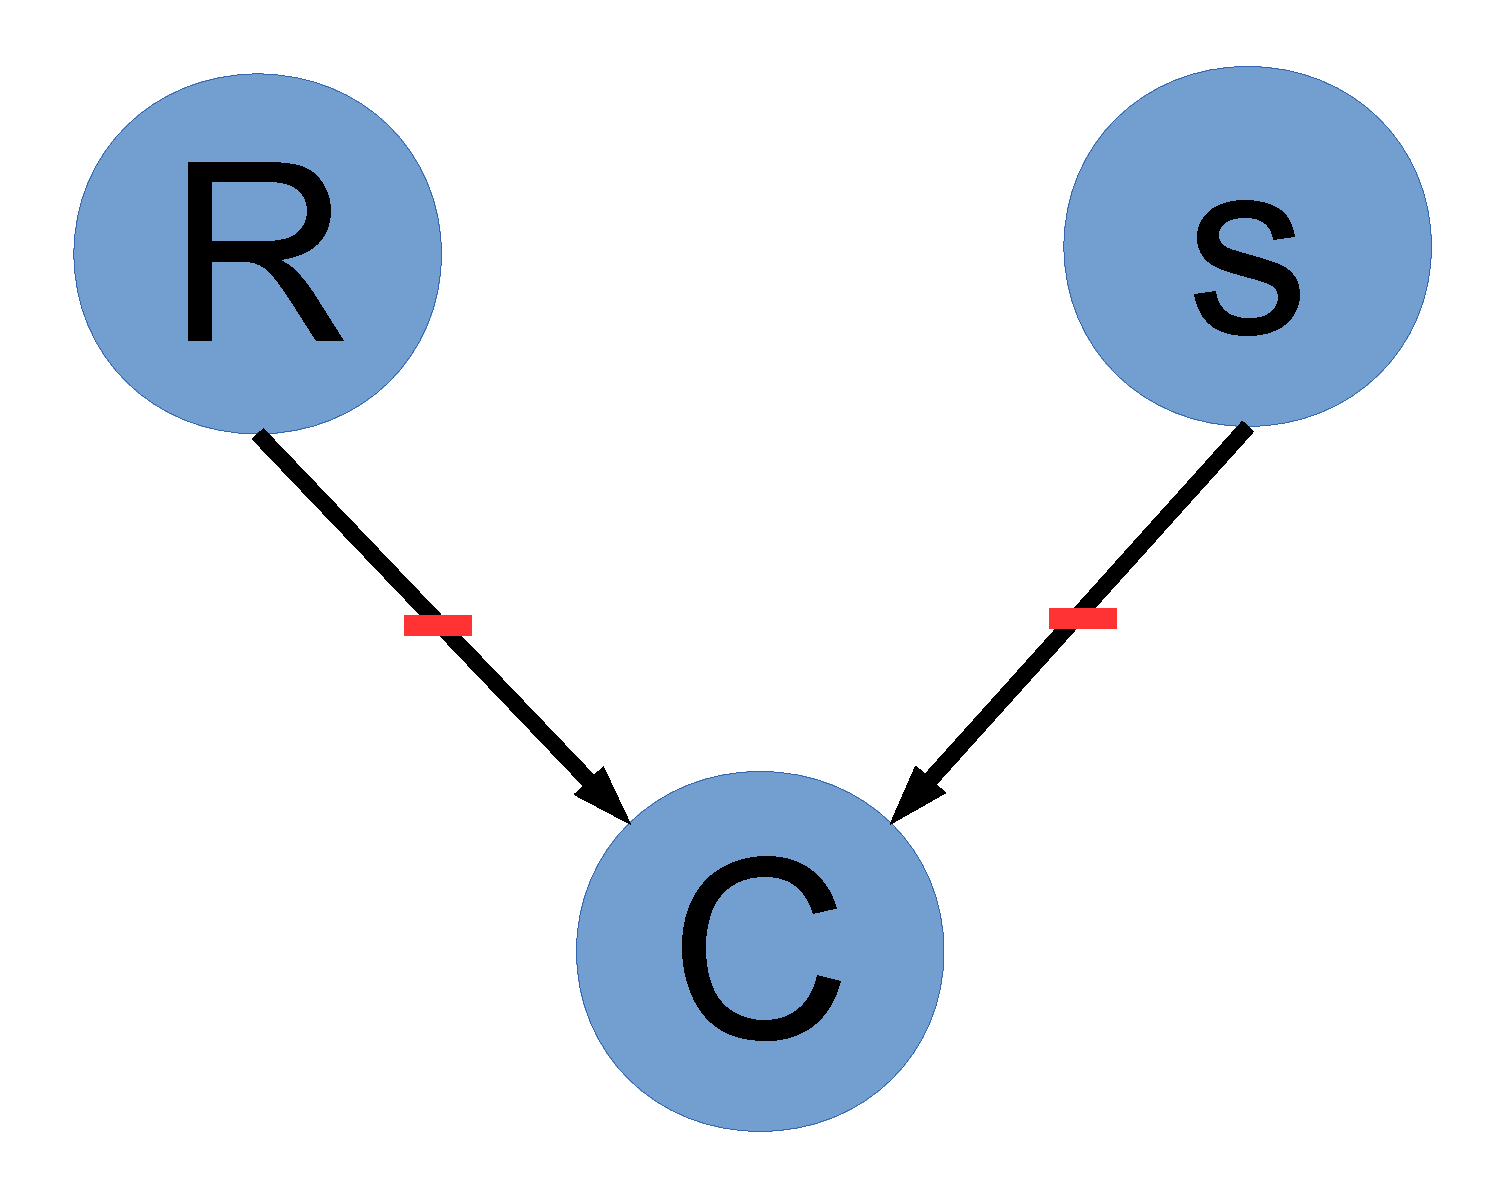
\includegraphics[width=\textwidth]{bernanke.pdf}
                \caption{\footnotesize Bernanke}
                \label{fig:bernanke}
        \end{subfigure}%
        ~ %add desired spacing between images, e. g. ~, \quad, \qquad etc.
          %(or a blank line to force the subfigure onto a new line)
        \begin{subfigure}[b]{0.2\textwidth}
                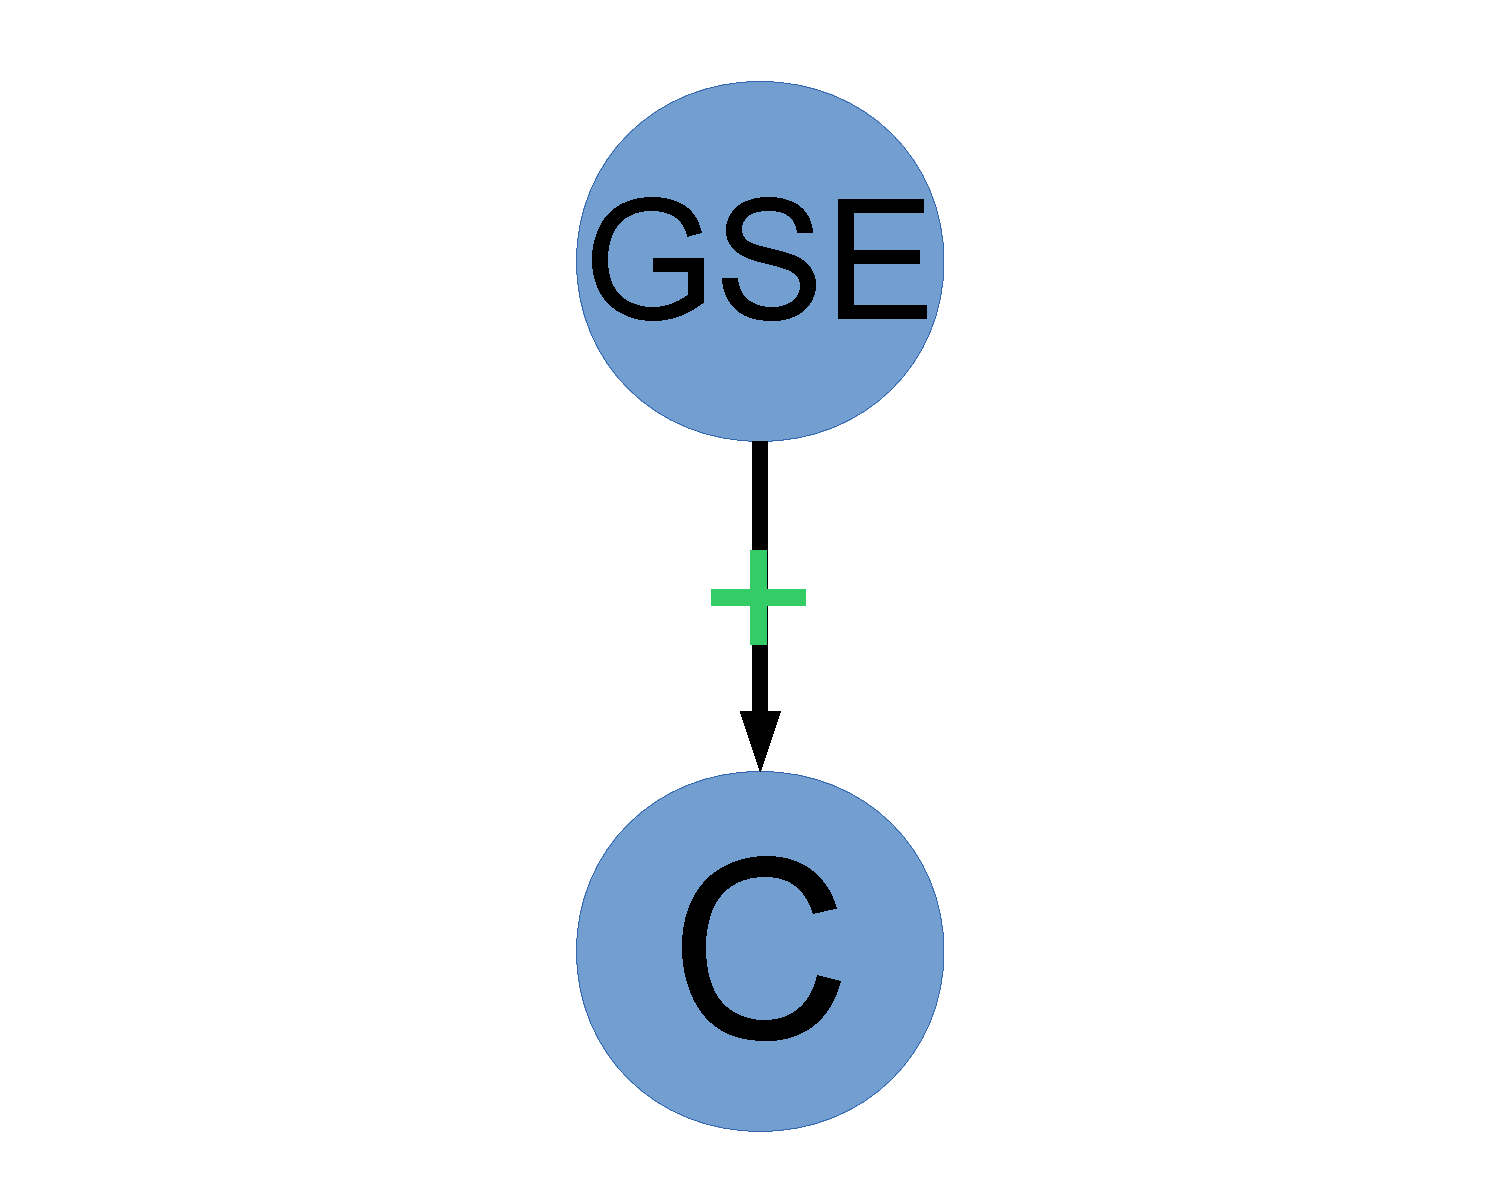
\includegraphics[width=\textwidth]{paulson.pdf}
                \caption{\footnotesize Paulson}
                \label{fig:paulson}
        \end{subfigure}
        \begin{subfigure}[b]{0.2\textwidth}
                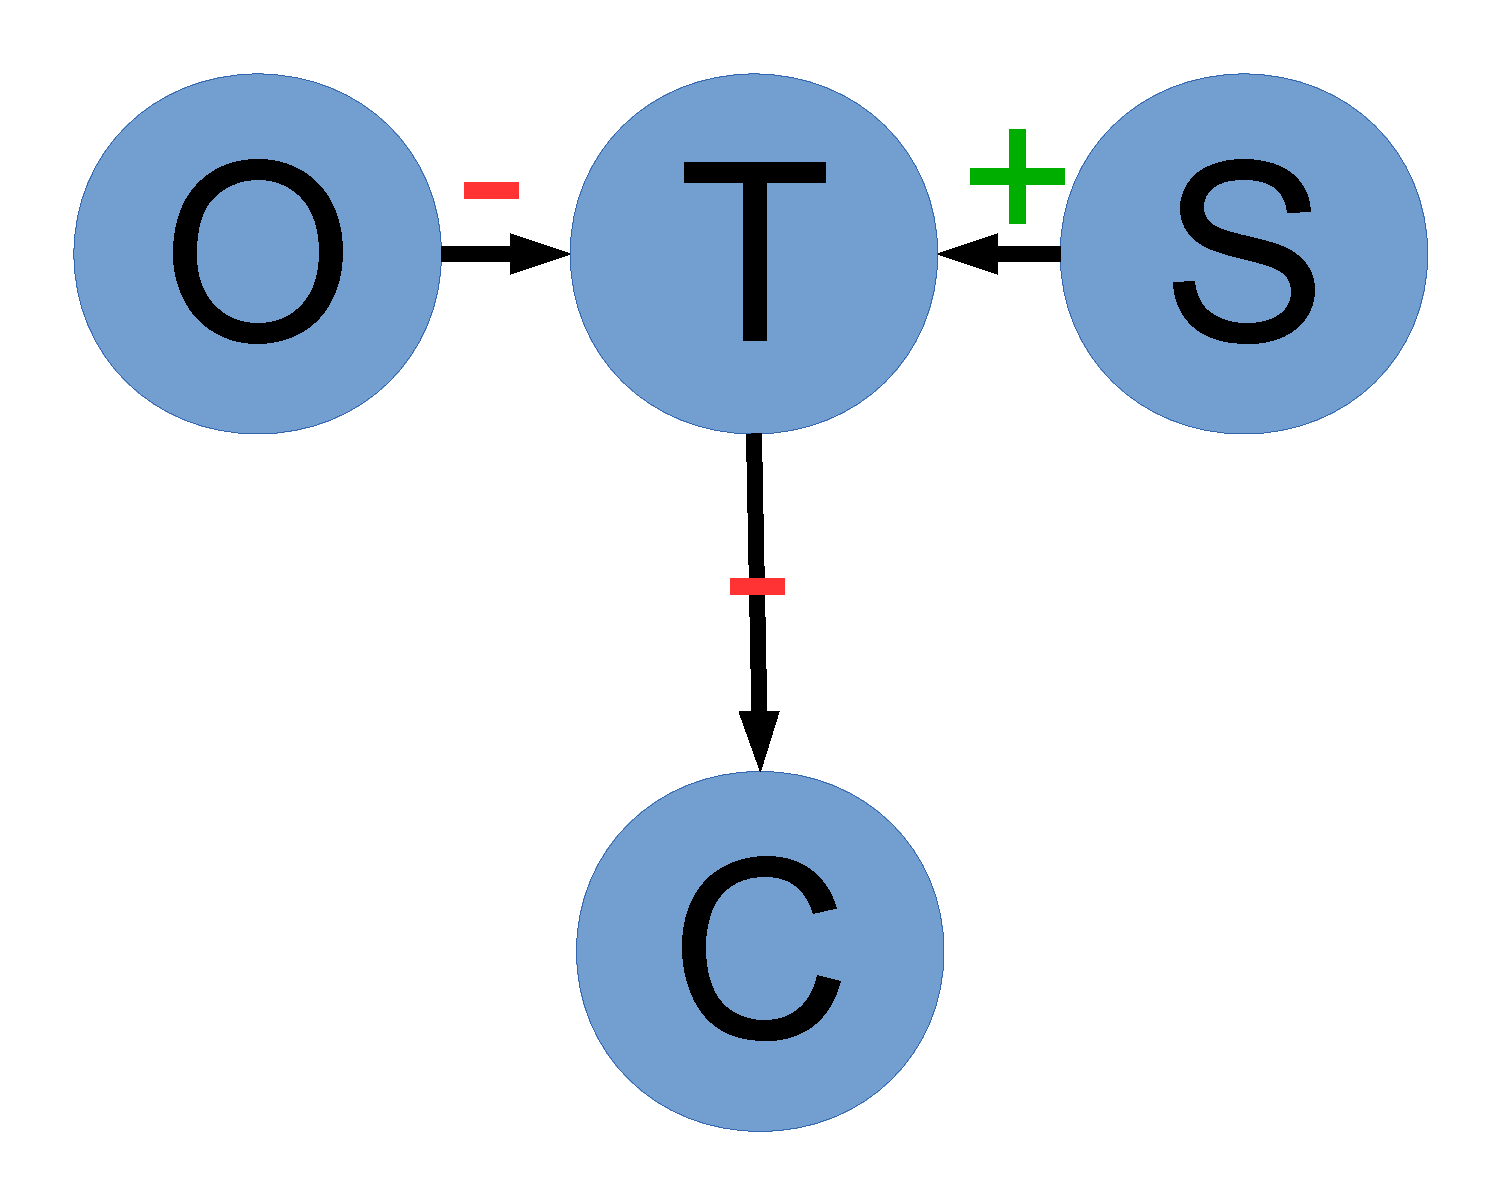
\includegraphics[width=\textwidth]{morgenthau.pdf}
                \caption{\footnotesize Morgenthau}
                \label{fig:morgenthau}
        \end{subfigure}
        \begin{subfigure}[b]{0.2\textwidth}
                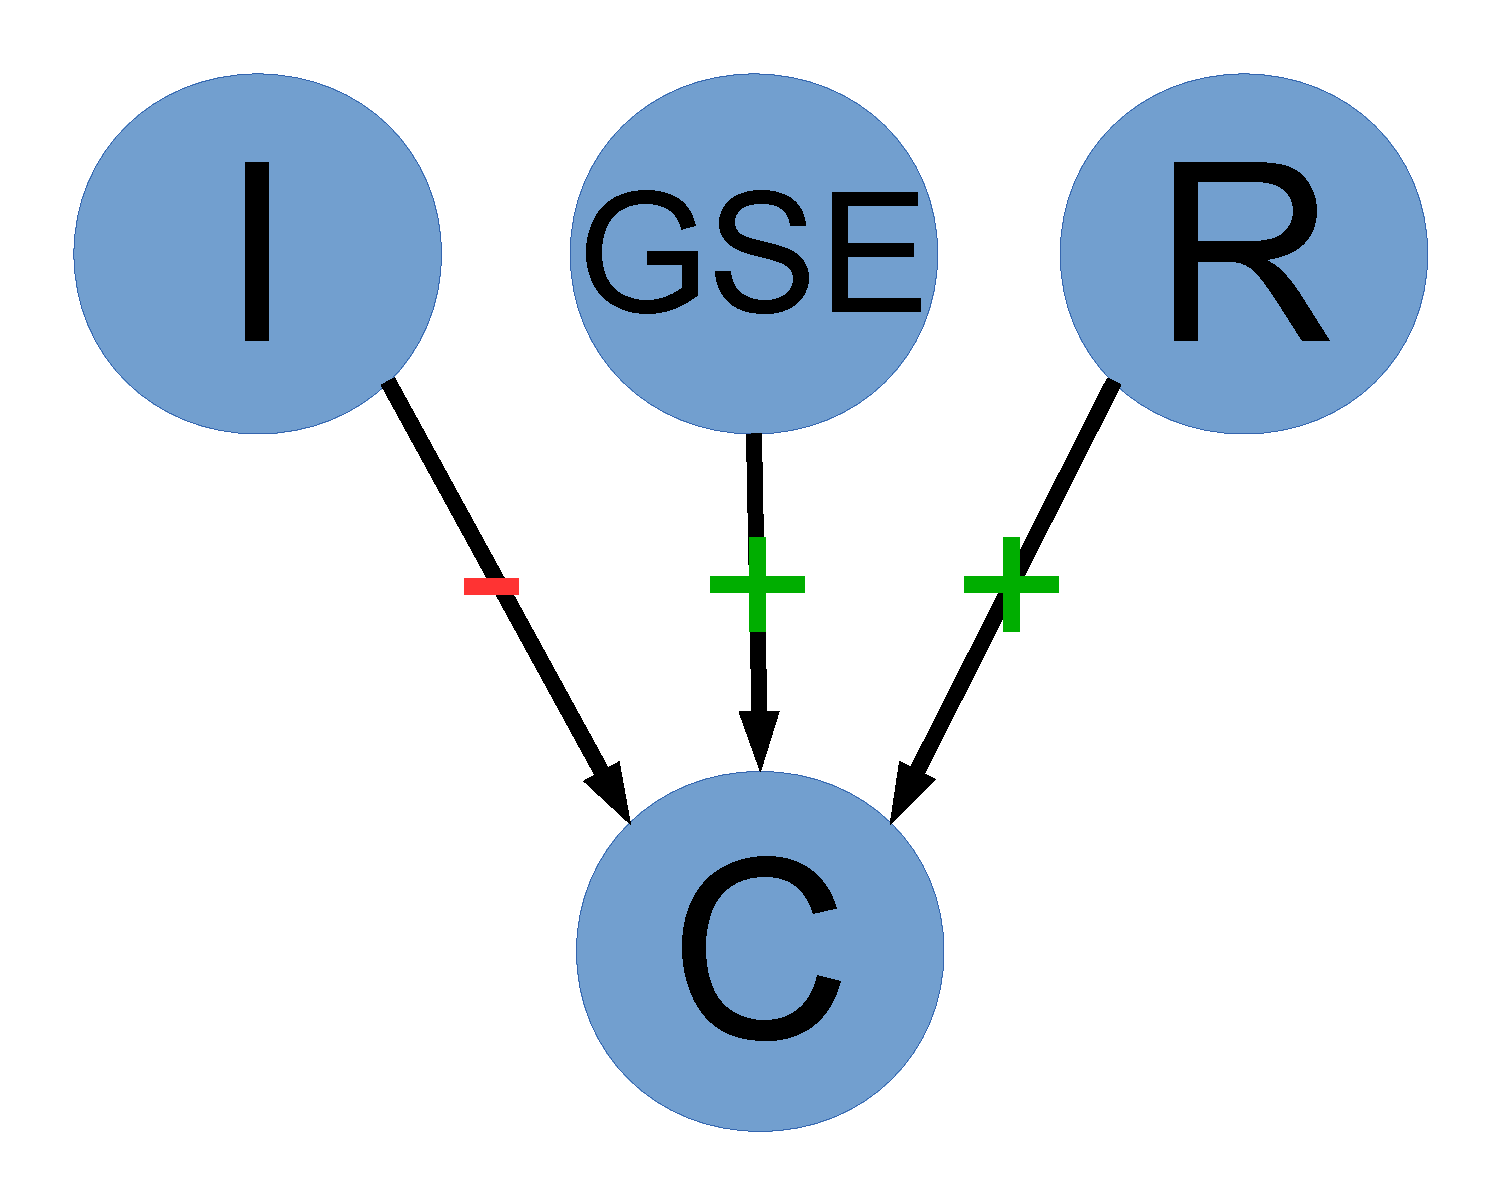
\includegraphics[width=\textwidth]{becker.pdf}
                \caption{\footnotesize Becker}
                \label{fig:becker}
        \end{subfigure}
        \begin{subfigure}[b]{0.2\textwidth}
                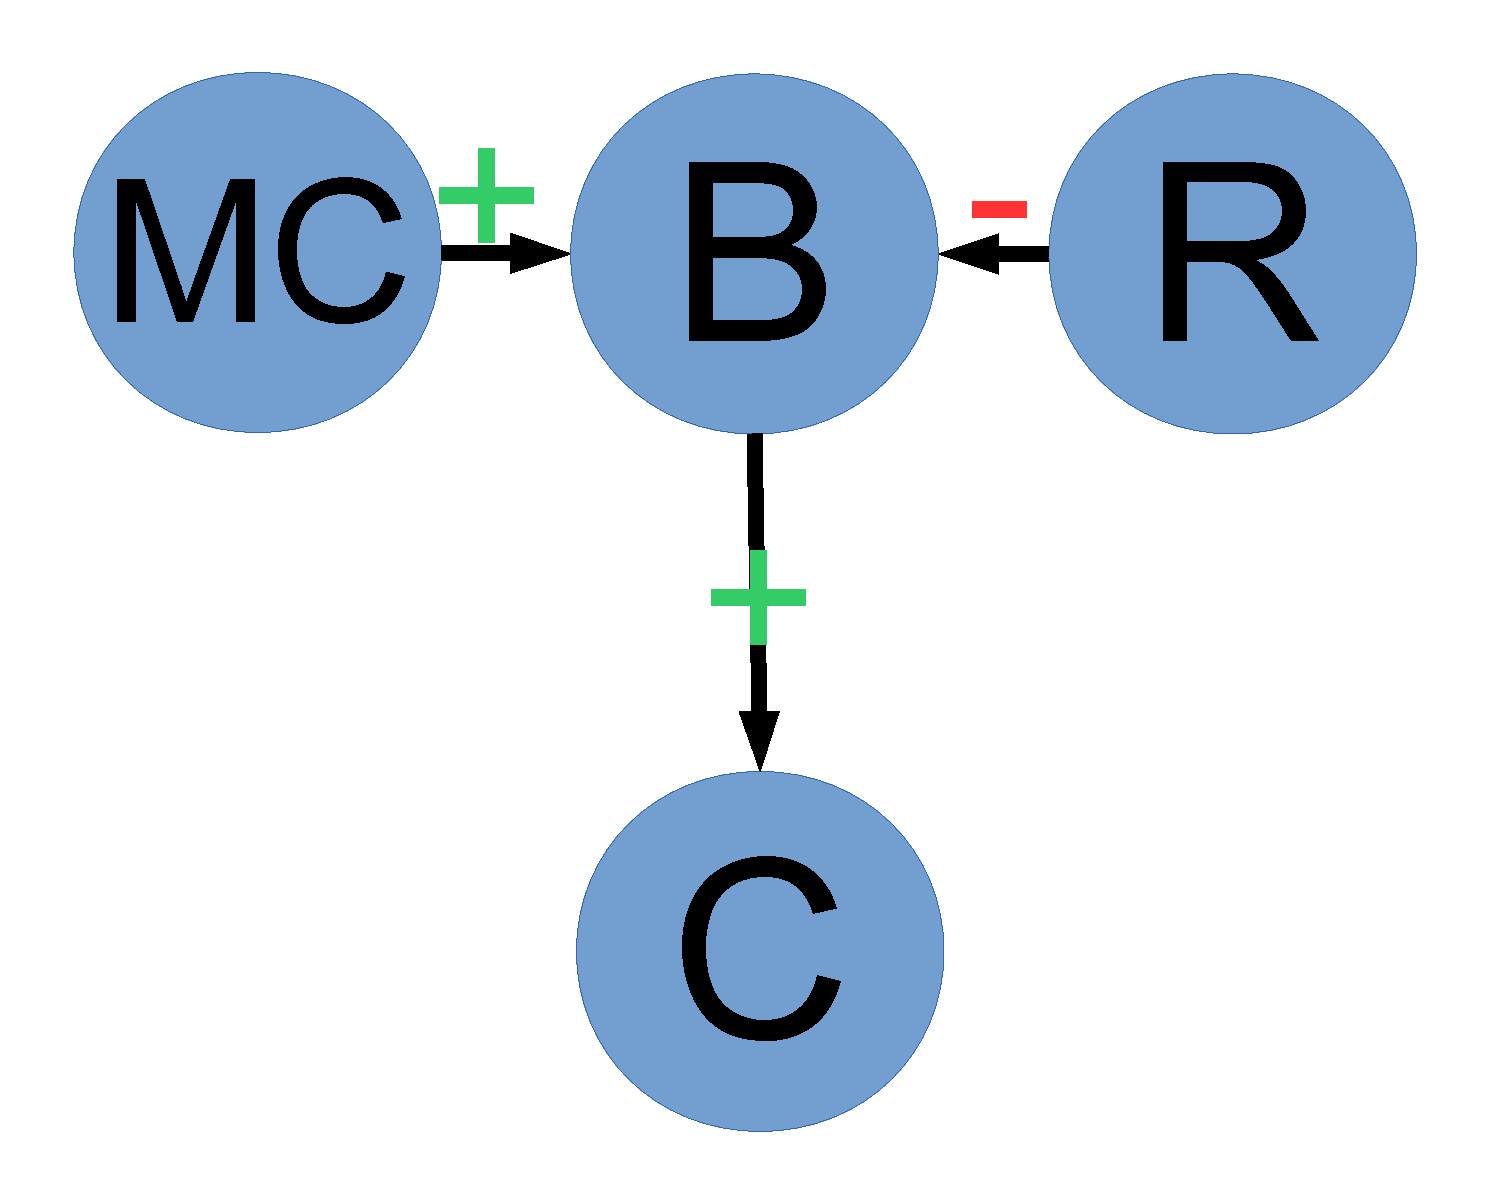
\includegraphics[width=\textwidth]{stiglitz.pdf}
                \caption{\footnotesize Stiglitz}
                \label{fig:stiglitz}
        \end{subfigure}
        \begin{subfigure}[b]{0.2\textwidth}
                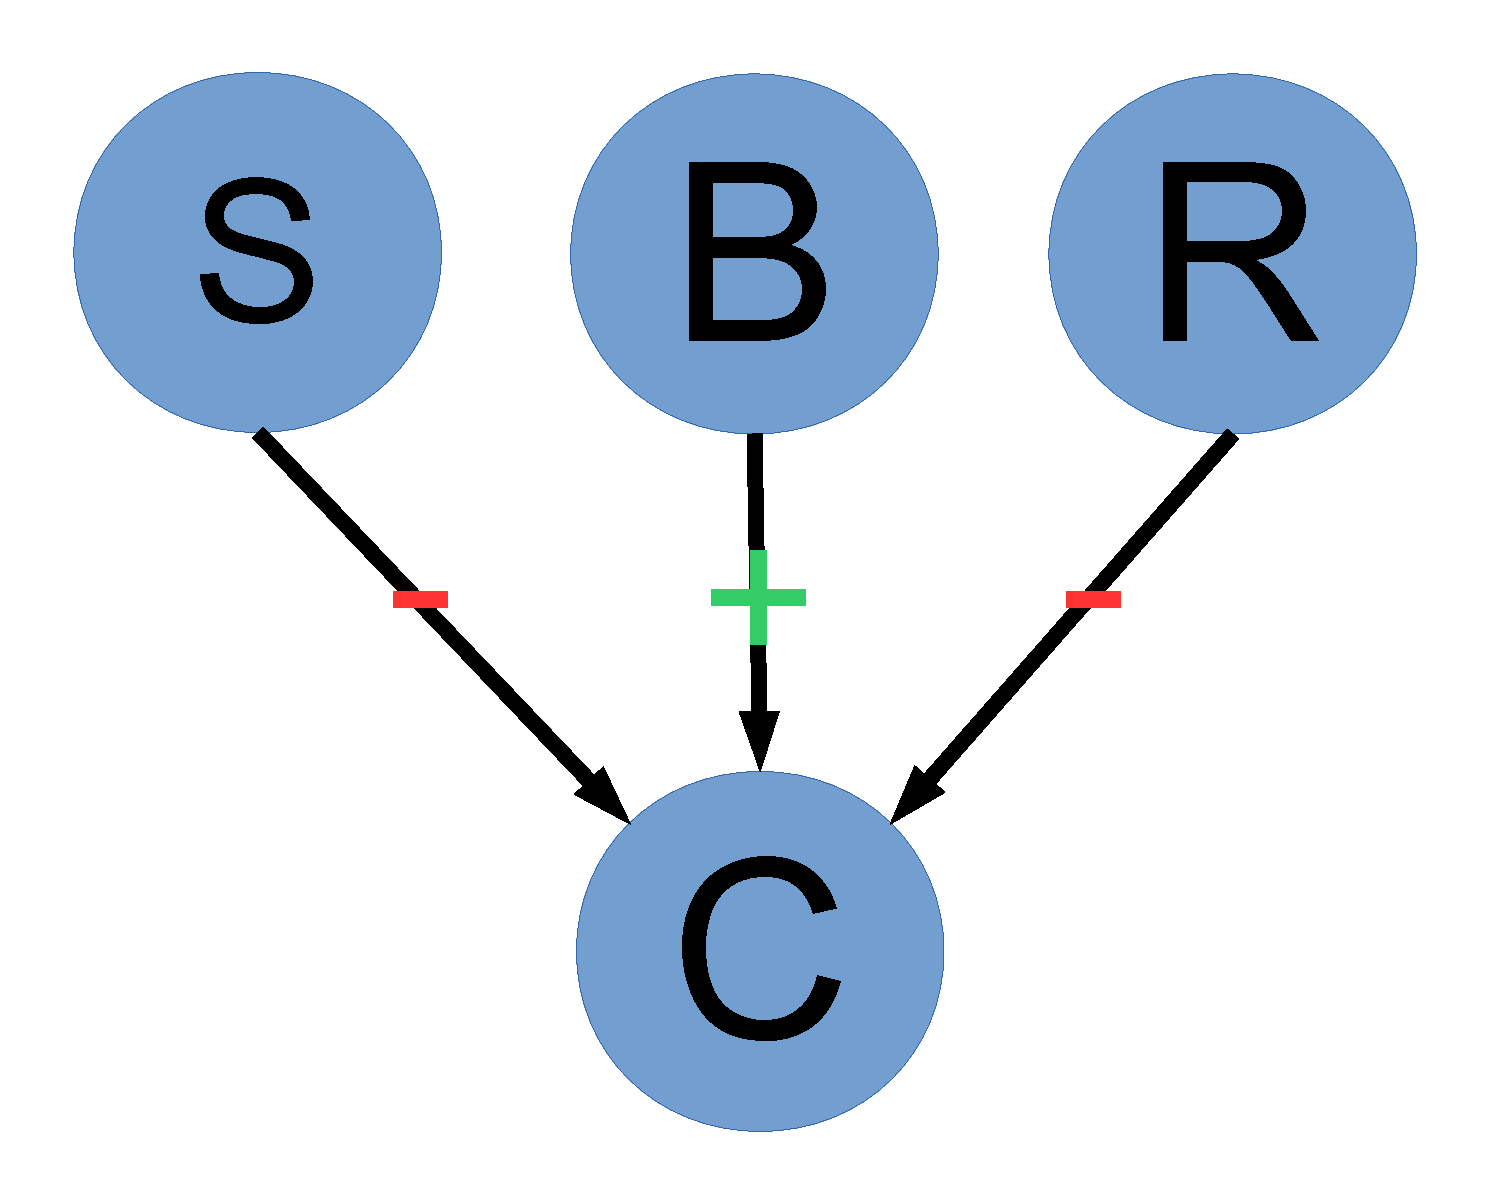
\includegraphics[width=\textwidth]{born.pdf}
                \caption{\footnotesize Born}
                \label{fig:born}
        \end{subfigure}
         \begin{subfigure}[b]{0.2\textwidth}
                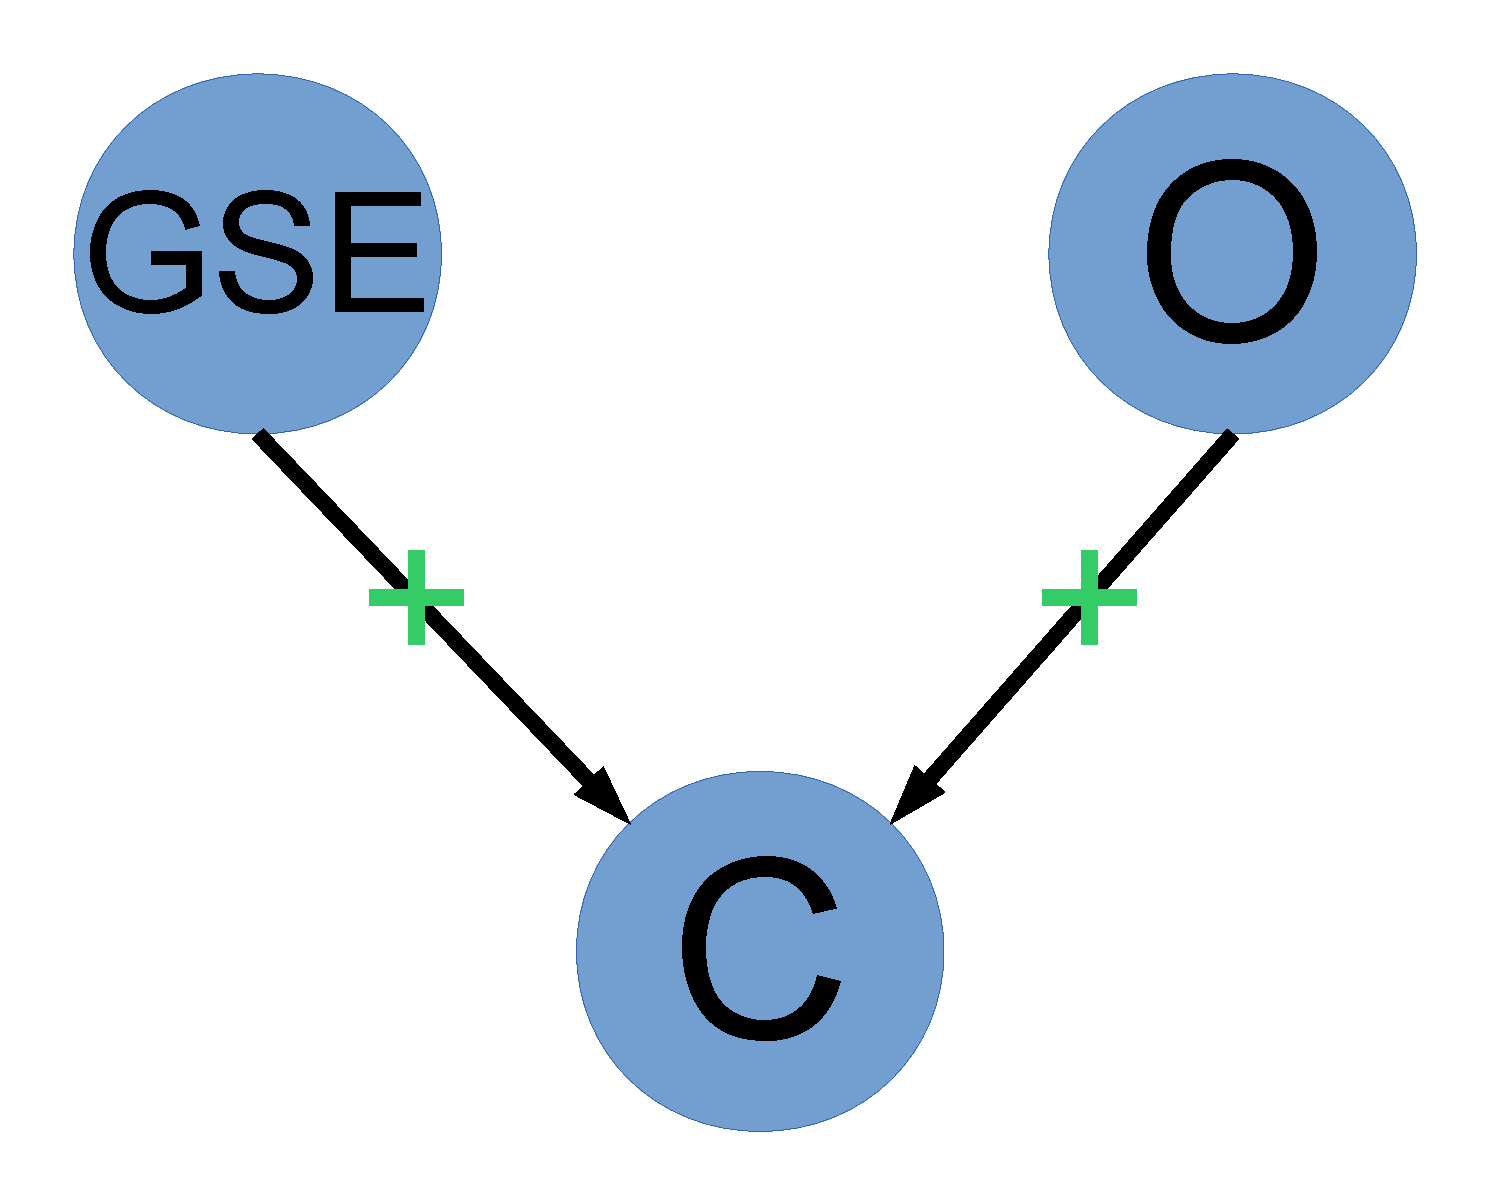
\includegraphics[width=\textwidth]{greenspan.pdf}
                \caption{\footnotesize Greenspan}
                \label{fig:greenspan}
        \end{subfigure}
        \begin{subfigure}[b]{0.2\textwidth}
                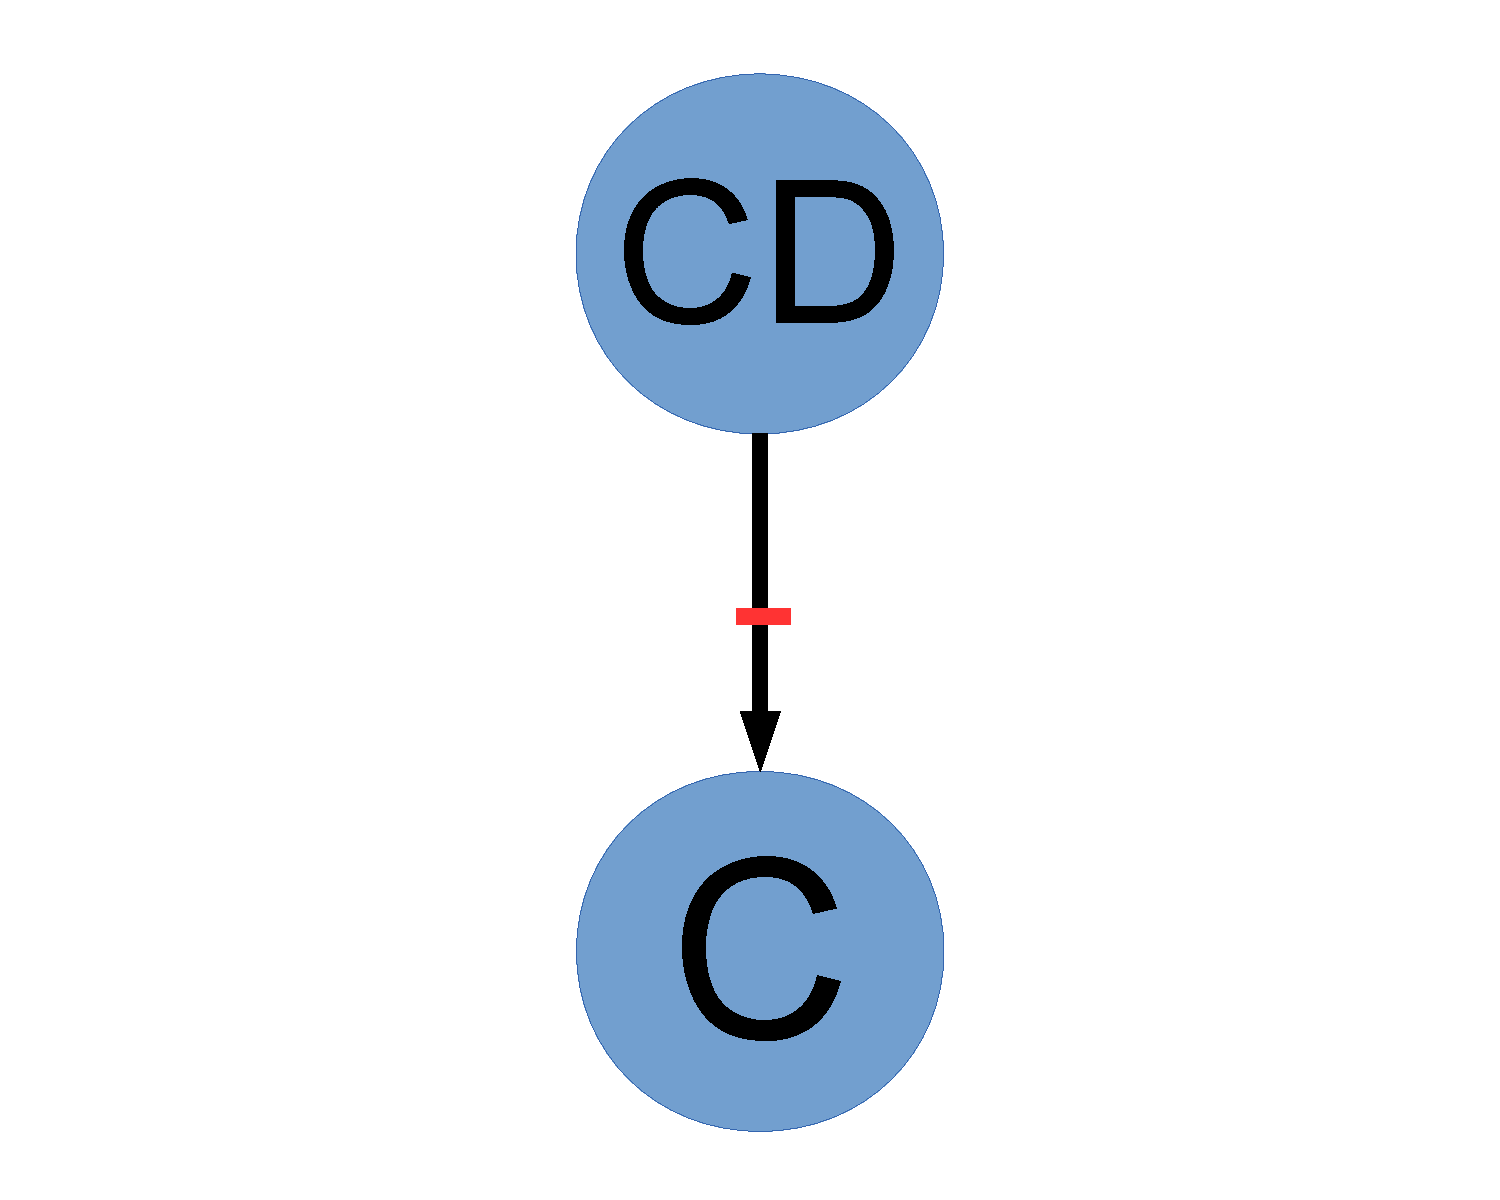
\includegraphics[width=\textwidth]{buffett.pdf}
                \caption{\footnotesize Buffett}
                \label{fig:buffett}
        \end{subfigure}
        \begin{subfigure}[b]{0.2\textwidth}
                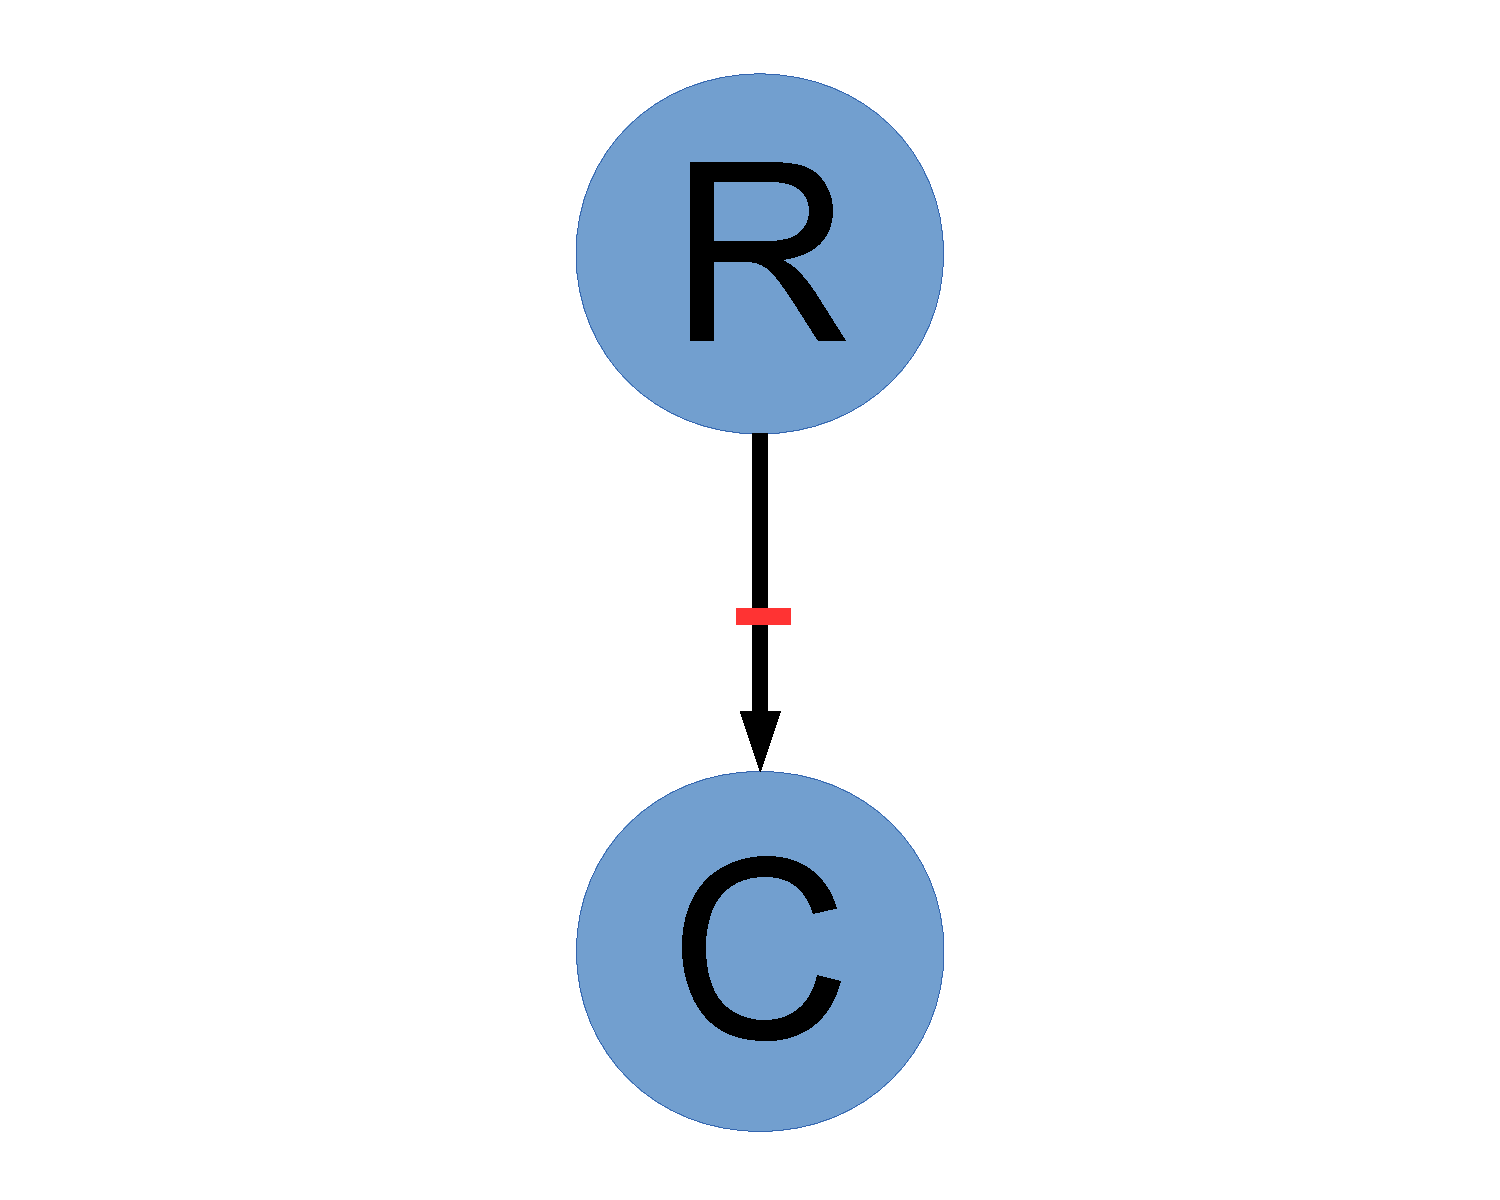
\includegraphics[width=\textwidth]{krugman.pdf}
                \caption{\footnotesize Krugman}
                \label{fig:krugman}
        \end{subfigure}
        \begin{subfigure}[b]{0.2\textwidth}
                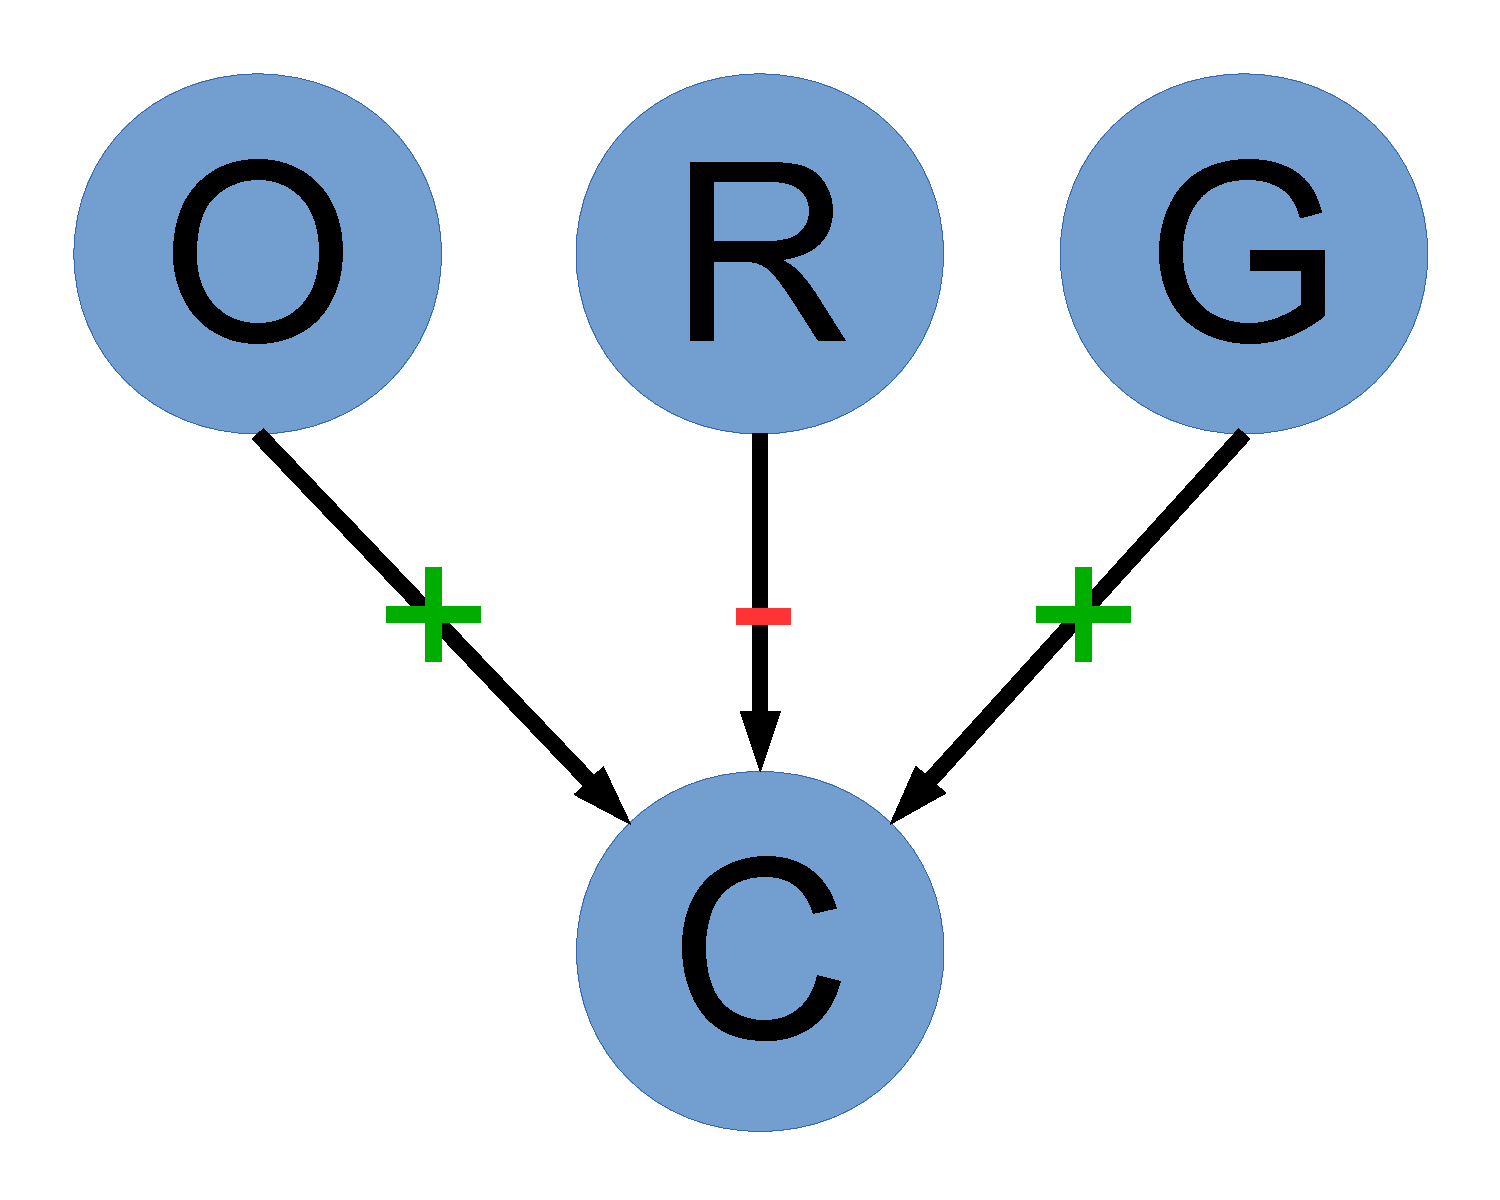
\includegraphics[width=\textwidth]{rodrik.pdf}
                \caption{\footnotesize Rodrik}
                \label{fig:rodrik}
        \end{subfigure}
        \begin{subfigure}[b]{0.2\textwidth}
                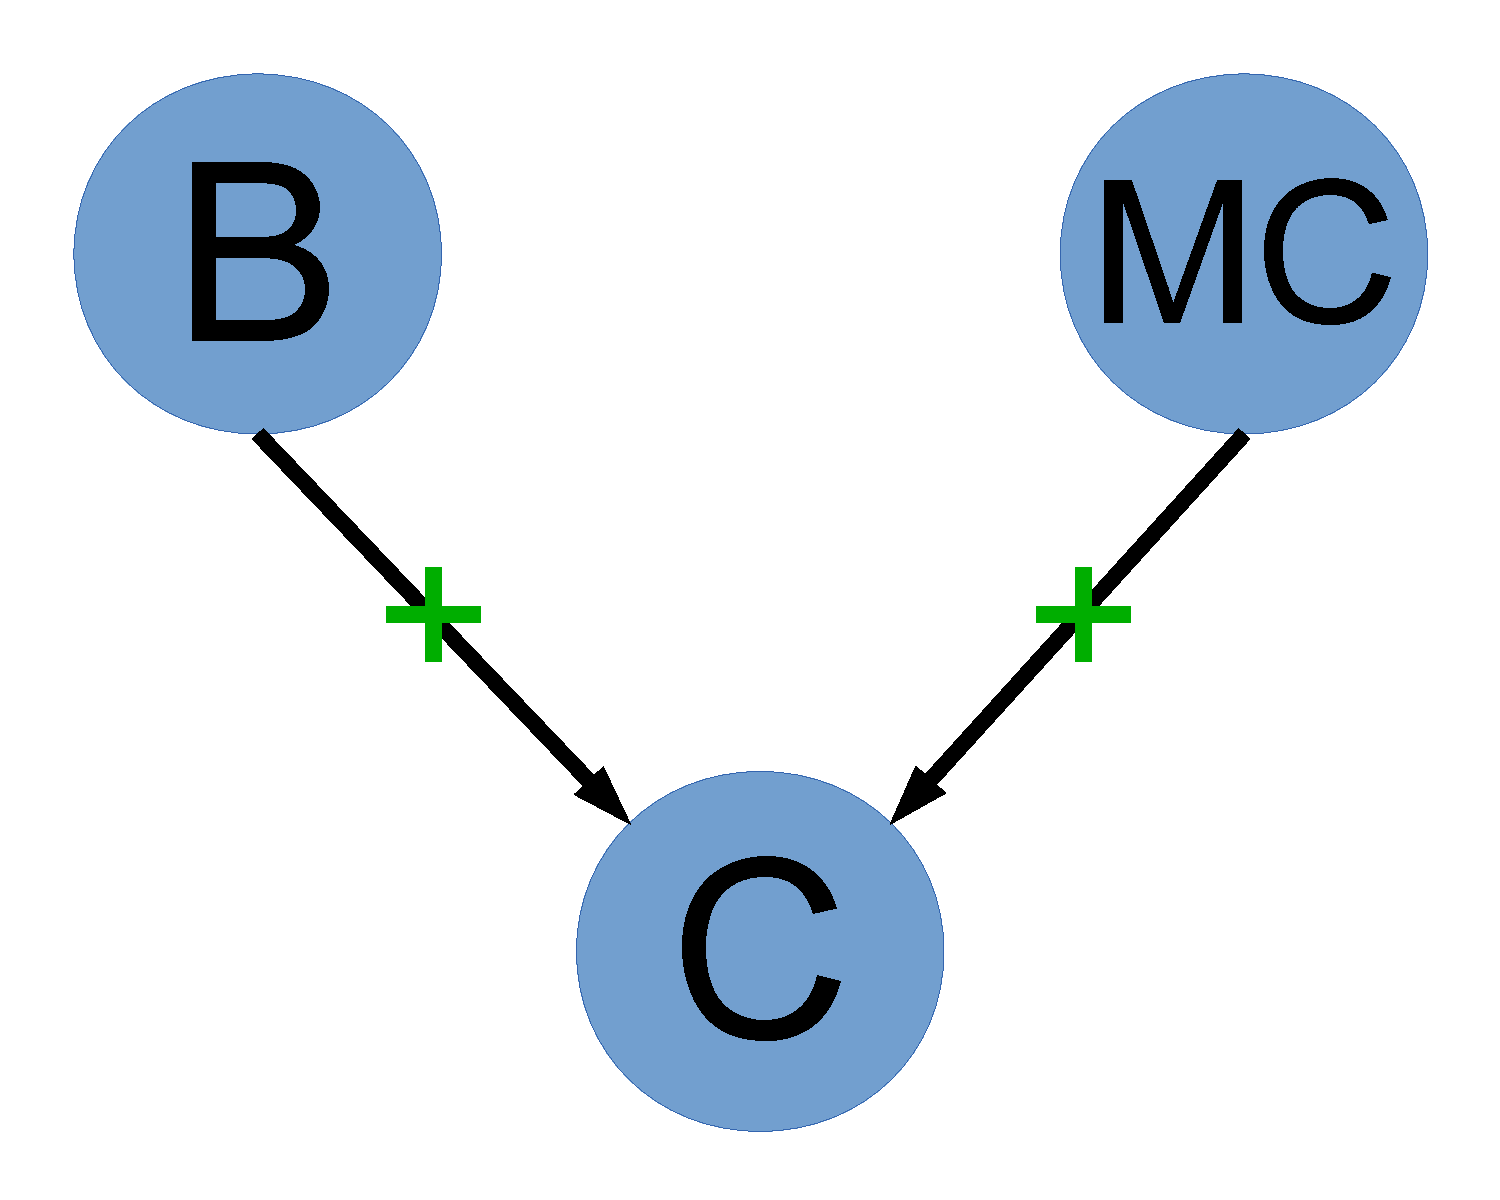
\includegraphics[width=\textwidth]{soros.pdf}
                \caption{\footnotesize Soros}
                \label{fig:soros}
        \end{subfigure}
        ~ %add desired spacing between images, e. g. ~, \quad, \qquad etc.
          %(or a blank line to force the subfigure onto a new line)
       \caption{$C$: Crisis, $R$: Regulation, $S$: Supervision, $I$: Interest Rate, $T$: Transparency, $O$: Offshoring, $GSE$: Government Promotion of Home-Ownership, $B$: Banking Behavior,  $MC$: Misguided Incentives, $CD$: Cognitive Diversity}\label{fig:committe1}
\end{figure}

\subsection*{The cast of characters is as follows:}
\begin{itemize}
\item Ben Bernanke (economist and chairman of the US Federal Reserve Bank, Figure ~\ref{fig:bernanke}),
\item Henry Paulson, Jr. (past CEO of Goldman Sachs and Secretary of the US Treasury at the time of the crisis, Figure ~\ref{fig:paulson}),
\item Robert Morgenthau, (District Attorney for New York County at the time of the crisis, Figure ~\ref{fig:morgenthau}),
\item Joseph Stiglitz (economist, Figure ~\ref{fig:stiglitz}),
\item Brooksley Born (Commissioner on the Financial Crisis Inquiry Commission and past chair of the Commodity Futures Trading Commission, Figure ~\ref{fig:born}),
\item Alan Greenspan (economist and past chairman of the US Federal Reserve Bank, Figure ~\ref{fig:greenspan}),
\item Warren Buffett (CEO and largest shareholder of Berkshire Hathaway, known as the ``Oracle of Omaha'', Figure ~\ref{fig:buffett}),
\item Paul Krugman (economist, Figure ~\ref{fig:krugman}),
\item Dani Rodrik (economist, Figure ~\ref{fig:rodrik})
and
\item George Soros (Chairman of Soros Fund Management and philanthropist, Figure ~\ref{fig:soros}).
\end{itemize}

\subsection*{Cognitive Distances}

\begin{table}[h]\hspace*{-3.5cm}
\centering
\footnotesize
\begin{tabular}{l*{10}{c}r}
Committee &   Bernanke   &   Paulson   &   Morgenthau   &   Becker   &   Stiglitz   &   Born   &   Greenspan   &   Buffett   &   Krugman   &   Rodrik   &   Soros\\
\hline
Bernanke     & 0.0    &        &        &        &        &        &        &        &        &        &       \\
Paulson      & 0.3483 & 0.0    &        &        &        &        &        &        &        &        &       \\
Morgenthau   & 0.3791 & 0.3778 & 0.0    &        &        &        &        &        &        &        &       \\
Becker       & 0.3592 & 0.3394 & 0.4345 & 0.0    &        &        &        &        &        &        &       \\
Stiglitz     & 0.3965 & 0.3783 & 0.4295 & 0.4651 & 0.0    &        &        &        &        &        &       \\
Born         & 0.1823 & 0.3968 & 0.4209 & 0.3162 & 0.3999 & 0.0    &        &        &        &        &       \\
Greenspan    & 0.3104 & 0.2415 & 0.3791 & 0.2636 & 0.4134 & 0.3151 & 0.0    &        &        &        &       \\
Buffett      & 0.3483 & 0.3128 & 0.3778 & 0.3968 & 0.3783 & 0.3968 & 0.3483 & 0.0    &        &        &       \\
Krugman      & 0.2415 & 0.3128 & 0.3778 & 0.447 & 0.3465 & 0.3394 & 0.3483 & 0.3128 & 0.0     &        &       \\
Rodrik       & 0.2636 & 0.3968 & 0.4209 & 0.3162 & 0.4472 & 0.238 & 0.2636 & 0.3968 & 0.3394 & 0.0 &           \\
Soros        & 0.3104 & 0.3483 & 0.399 & 0.3151 & 0.3198 & 0.2636 & 0.3104 & 0.3483 & 0.3483 & 0.3151 & 0.0\\
\hline
\multicolumn{12}{|c|}{After adjustment for Joseph Stiglitz:} \\
\hline
Stiglitz & 0.2636 & 0.3968 & 0.4345 & 0.3162 & 0.0 & 0.1764 & 0.3151 & 0.3968 & 0.3394 & 0.238 & 0.1823
\end{tabular} \hspace*{-3.5cm}
\caption{The pair-wise cognitive distance measure, $\sqrt{\text{JSD}_2(i, j)}$, for each pair of experts.} \label{table:cogndist}
\end{table}

Table ~\ref{table:cogndist} shows the Cognitive Distance, $\sqrt{\text{JSD}_2(i, j)}$, between any two experts. The five largest distances are, in order from greatest to lowest magnitude, those between 1) Stiglitz and Becker (0.465), 2) Stiglitz and Rodrik (0.447), 3) Krugman and Becker (0.447), 4) Morgenthau and Becker (0.4345) and 5) Stiglitz and Morgenthau (0.429). The cognitive maps of both, Joseph Stiglitz (Figure ~\ref{fig:stiglitz}) and Gary Becker (Figure ~\ref{fig:becker}) are present in three out of the five largest diadic distances, while that of Robert Morgenthau (Figure ~\ref{fig:morgenthau}) is involved in two of the five largest distances. The maps of Stiglitz and Morgenthau are structurally more complex than all others in the collection, in that they both include a mediating variable through which two other variables causally affect the onset of the crisis, instead of being composed of $1$ to $3$ direct causes which is the case of all other maps. Also, Morgenthau's map includes a variable, $T$ (transparency) that is absent from all other maps, while Stiglitz's map includes a variable $MC$ (misguided incentives) which is present in only one other map (Soros's, Figure ~\ref{fig:soros}). Gary Becker's map is unique in that it includes a \textit{positive} causal relation from $R$ (financial regulation) to the onset of the crisis, $C$, while all others who considered $R$ argued that its lack was responsible and not that there was too much of it. Becker stated that the regulators were in part to be blamed for the crisis, as they were ``cheerleaders for the banks,'' and it is important to note that my choice to code Becker's partial blame on the regulators as a positive causal relation from $R$ to $C$ is debatable. Indeed, $R$ might not be the right variable, if $R$ is the symbol that is used for all others to denote the quantity of regulation, and what might be needed is an additional variable $RB$ (the behavior of the regulators). In order to keep a bound on the number of variables (to keep things simple) I choose to code Becker's statement as $R \xrightarrow{+} C$, with the explicit caveat that this assumption might cause to exaggerate the magnitudes of some of my measures.

The five shortest distances, in order of increasing magnitude, are between 1) Bernanke and Born (0.182), 2) Rodrik and Born (0.238), 3) Bernanke and Krugman (0.241), 4) Greenspan and Paulson (0.241) and 5) Becker and Greenspan, Rodrik and Greenspan, Bernanke and Rodrik and Born and Soros (all with distance 0.2636). The shortest cognitive distance is that between Ben Bernanke (Figure ~\ref{fig:bernanke}) and Brooksley Born (Figure ~\ref{fig:born}), whose cognitive maps are essentially the same, except that Born's map includes one additional positive edge from $B$, the behavior of the banks, to the onset of the crisis, $C$. The second shortest cognitive distance, that between Dani Rodrik (Figure ~\ref{fig:rodrik}) and Brooksley Born (Figure ~\ref{fig:born}), is already much greater in magnitude; it is by a factor of $1.3$ greater than the smallest, where the maximum distance is by a factor of about $2.6$ greater. This jump in magnitude, from the shortest to the second shortest distance is no surprise when one looks at the two graphs involved in the calculation; Rodrik's and Born's maps have one causal relation in common and are similar in structure, but each has two causes that the other has not.

\subsection*{Sensitivity of the Measures}

\begin{figure}
        \centering
        \begin{subfigure}[b]{0.2\textwidth}
                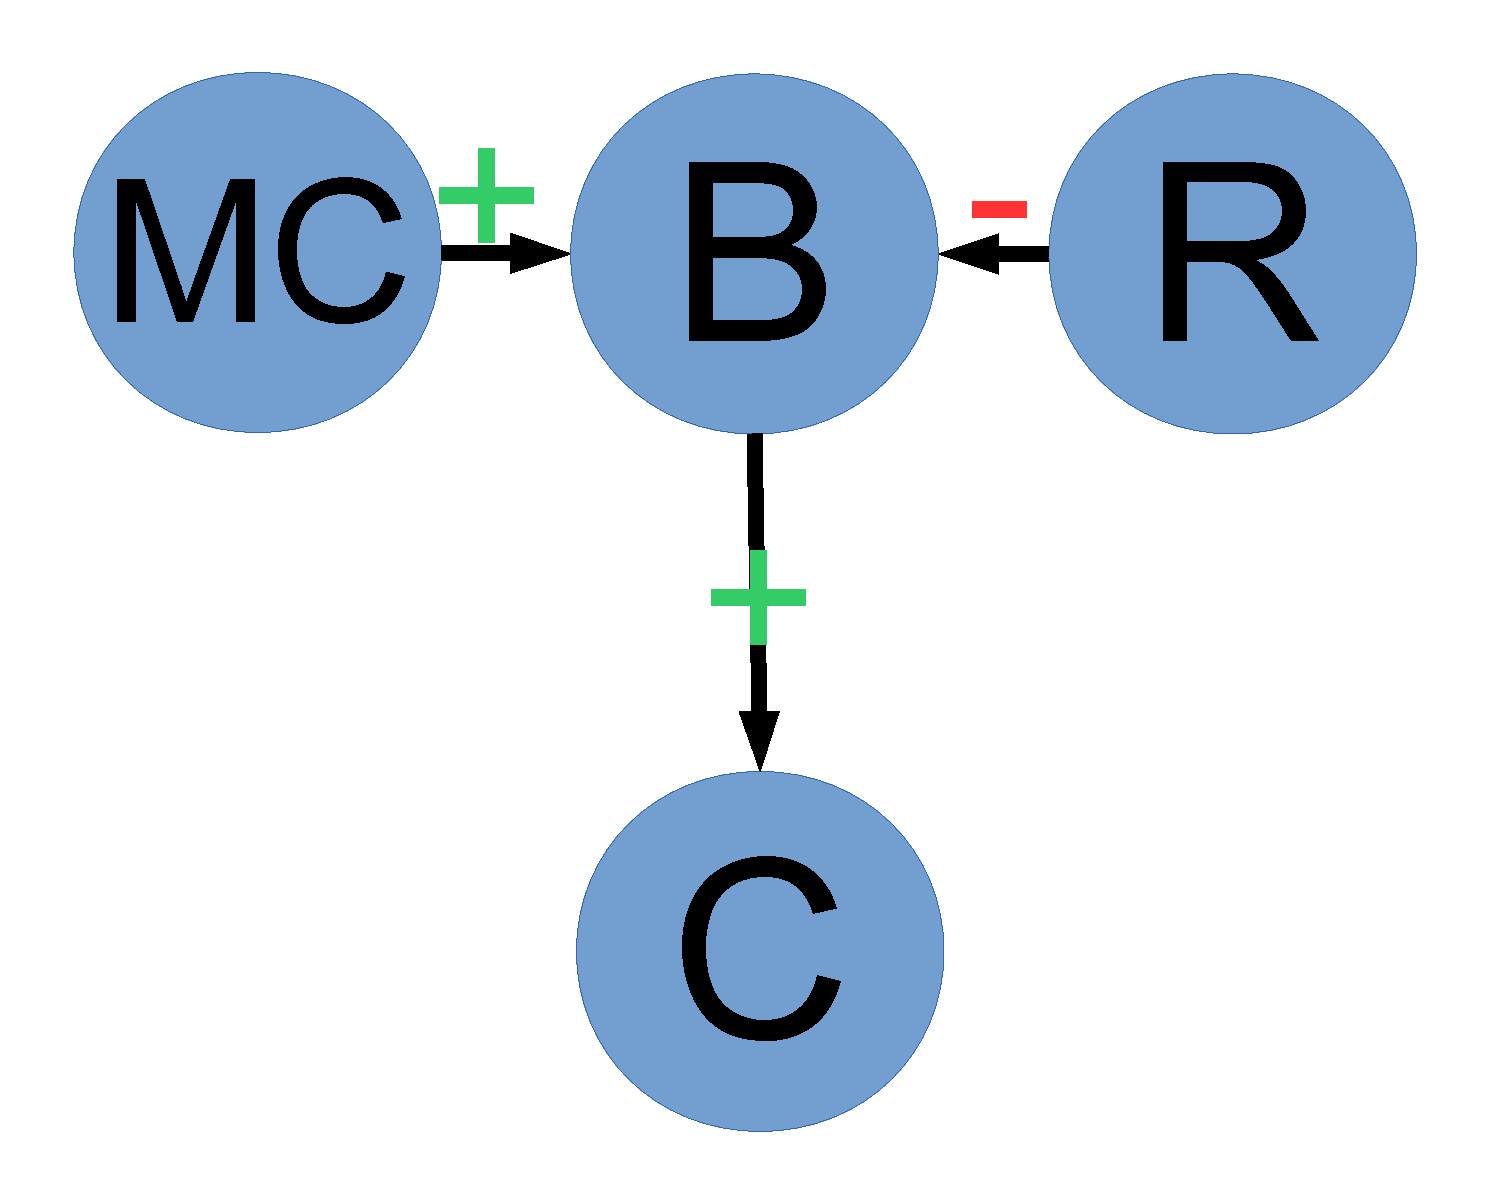
\includegraphics[width=\textwidth]{stiglitz.pdf}
                \caption{\footnotesize Stiglitz (before adjustment)}
                \label{fig:before}
        \end{subfigure}%
        ~ %add desired spacing between images, e. g. ~, \quad, \qquad etc.
          %(or a blank line to force the subfigure onto a new line)
        \begin{subfigure}[b]{0.2\textwidth}
                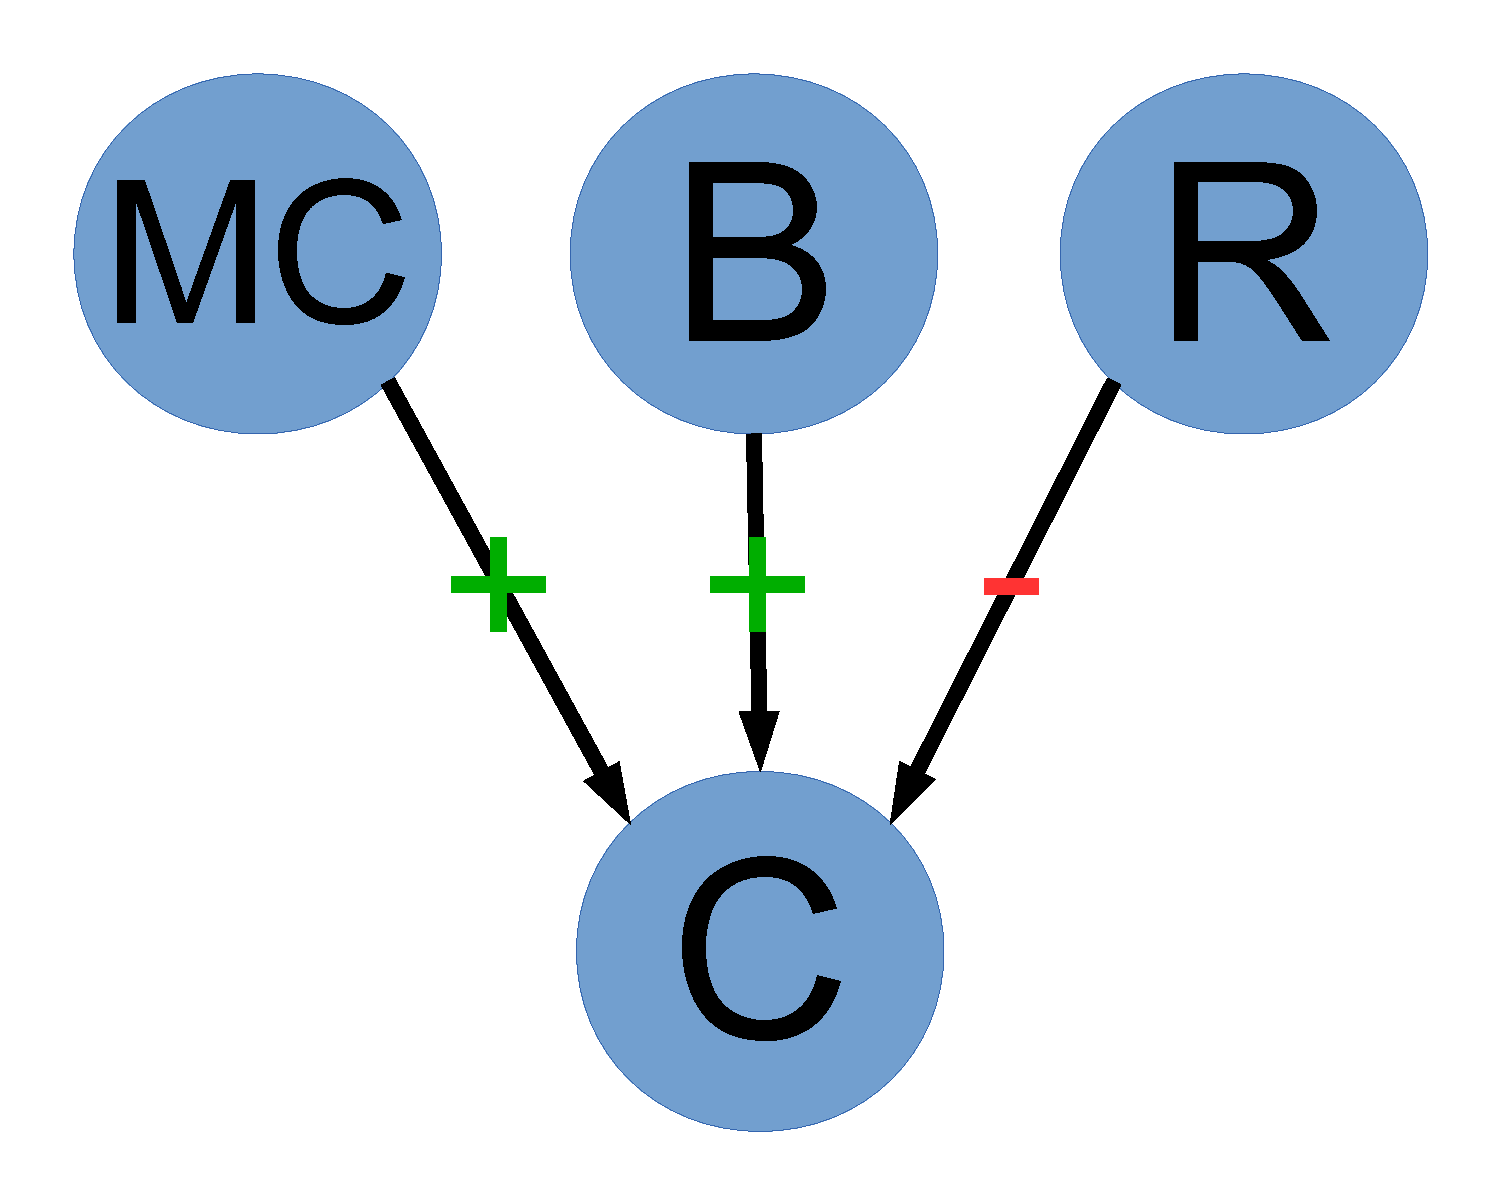
\includegraphics[width=\textwidth]{stiglitz2.pdf}
                \caption{\footnotesize Stiglitz (after adjustment)}
                \label{fig:after}
        \end{subfigure}
\caption{A plausible simplification of Joseph Stiglitz's CM, variables are: $C$: Crisis, $R$: Regulation, $B$: Banking Behavior,  $MC$: Misguided Incentives.}\label{fig:adjustment}
\end{figure}


It is important to experiment with these measures in order to get a better understanding of their meaning. For example, with these representations of beliefs, Joseph Stiglitz might be further removed in distance than is truly warranted, from Born, Bernanke, Rodrik and Krugman, simply because his map includes behavior as a mediating variable, mediating between incentives as well as regulation and the onset of the crisis, where the others very likely have the same in mind but see this as too trivial to make explicit (hence their maps look very different). Making an adjustment that simplifies Joseph Stiglitz's map (see Figure ~\ref{fig:adjustment}), decreases the overall diversity measure, from $0.302$ to $0.289$. For Joseph Stiglitz, his distance to Bernanke decreases to $0.264$, his distance to Paulson increases to $0.397$, while the decrease of his distance to Born is most dramatic, decreasing from $0.4$ to $0.18$, an adjustment which makes them the closest in terms of cognitive distance for the whole collection. Thus, it is clear that these measures are very sensitive to the exact specification of beliefs and that therefore great care must be taken in the elicitation and processing of people's statements. However, I see this sensitivity as a strength, rather than a weakness of the measuring approach, as the diversity that results from differences in exact communication patterns and thoughts (such as the inclusion and exclusion of potentially important mediating variables), might be precisely what leads to a collective's greater understanding of the world.

\subsection*{Constructing Diverse Collectives}

\begin{table}[h]\hspace*{-3.5cm}
\centering
\footnotesize
\begin{tabular}{l*{10}{c}r}
Committee &   Bernanke   &   Paulson   &   Morgenthau   &   Becker   &   Stiglitz   &   Born   &   Greenspan   &   Buffett   &   Krugman   &   Rodrik   &   Soros\\
\hline
$n=10$     & -0.0112 & -0.0055 & 0.0054 & -0.0018 & 0.0058 & -0.0091 & -0.0107 & -0.003  & -0.006  & -0.007  & -0.0099  \\
$n=9$      &         & -0.0078 & 0.0049 & -0.0036 & 0.0049 & -0.0094 & -0.0135 & -0.0047 & -0.0067 & -0.0081 & -0.0125\\
$n=8$      &         & -0.009  &  0.004 & -0.0037 & 0.0027 & -0.0125 &         & -0.0073 & -0.0099 & -0.0094 & -0.0161\\
$n=7$      &         & -0.0133 & 0.0015 & -0.0049 & 0.0031 & -0.015  &         & -0.0111 & -0.0145 & -0.0126 &        \\
$n=6$      &         & -0.0206 &-0.0016 & -0.0037 & 0.002  &         &         & -0.0175 & -0.0192 & -0.0116 &        \\
\hline
$n=5$      &         &         &-0.0053 & -0.0041 & -0.0002&         &         & -0.0236 & -0.026  & -0.0213 &        \\
%\subsection{Notes}
\end{tabular} \hspace*{-3.5cm}
\caption{Morgenthau, Becker, Stiglitz, Buffett, Krugman and Rodrik survived the iterated deletion of diversity minimizing elements, for a maximally diverse group of 5. (the algorithm is as in Equation ~\ref{eq:min})} \label{table:minimize}
\end{table}

Interesting is also to measure how much each individual view of the crisis contributes to the diversity of the collection of views, so that an $l$ person team of experts can be constructed with the goal of maximizing diversity in mind (if that were to be found desirable)\footnote{In practice of course, there are many more conciderations aside from just cognitive diversity and it is likely never advisable to be entirely directed by such a uni-dimensional goal.}. There are two ways in which a maximally diverse group of, say $5$, could be constructed from a group of $10$: one way is to repeatedly subtract that person from the group whose presence contributes the least to (or subtracts the most from) the diversity of the group, (i.e. Equation ~\ref{eq:min}) and the other is to, starting from the cognitive distance of two people's graphs, repeatedly adding that additional person whose inclusion maximizes the cognitive diversity of the larger group (Equation ~\ref{eq:max}):
\begin{equation}\label{eq:min}
\min_i\left(\sqrt{\frac{JSD_n(\Omega_n)}{\log_2(n)}}-\sqrt{\frac{JSD_{n-1}(\Omega_n\setminus\text{Graph}_i)}{\log_2(n-1)}}\right), \text{ for } n=10, \ldots, 6,
\end{equation}
where $\Omega$ is the collection of all graphs and $\Omega\setminus\text{Graph}_i$ is the collection of all graphs, except Graph$_i$: the graph whose exclusion maximizes the diversity over the remaining $n-1$ graphs (see Table ~\ref{table:minimize} for an illustration).
\begin{equation}\label{eq:max}
\max_i\left(\sqrt{\frac{JSD_{\tau+1}(S_{\tau}\oplus\text{Graph}_i)}{\log_2(\tau+1)}}-\sqrt{\frac{JSD_{\tau}(S_{\tau})}{\log_2(\tau)}}\right), \text{ for }, \tau=1, \ldots, 4,
\end{equation}
where $S$ is initiated as one of those elements, with the largest cognitive distance in the group to some other element (here Joseph Stiglitz, before the adjustment) and then is incremented each time to maximize the diversity of $S_{\tau}\oplus\text{Graph}_i$, the collection that includes all members in $S$ and the additional member $i$, whose graph maximizes the diversity of the resulting collection with size $\tau + 1$.

\subsection*{Causal Intensity: the Parameters}

\begin{figure}
        \centering
        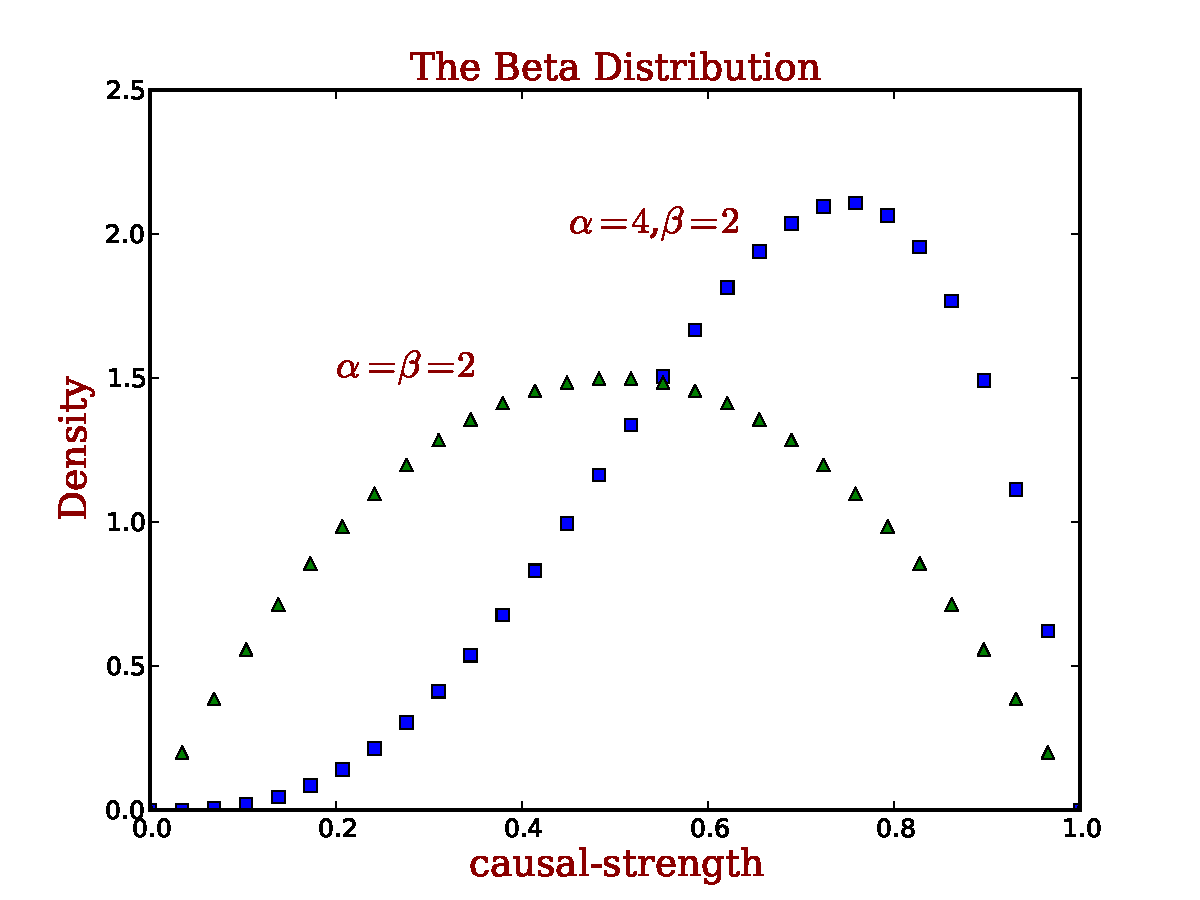
\includegraphics[width=80mm]{beta.pdf}
  \caption{The beta distribution for two different parameterizations $(\alpha, \beta)$.}
                \label{fig:beta}
        \end{figure}%

Recall that for any belief system (Graph$_i$), the probability of a data point, $D$, given the beliefs is calculated as

$$P(D | \text{Graph}_i)=\int_0^1 \hdots \int_0^1 P_i(D | \text{Graph}_i, \pi_{i, 0},\ldots, \pi_{i, k})P(\pi_{i, 0},\ldots, \pi_{i, k} | \text{Graph}_1) d\pi_{i, 0}\hdots d\pi_{i, k}$$

for $k$ causal effect parameters, where the ``Noisy-OR'' parameterization is used. The effect parameters themselves are drawn from the joint-distribution, $P(\pi_{i, 0}, \ldots, \pi_{i, k} | \text{Graph}_i)$, which in this case is simply the product of the marginals (I assume parameters to be drawn independently from their marginal distributions). Further, as a speaker's emphasis is harder to evaluate, I assume all effect parameters to be drawn from the same beta distribution, $B(\alpha, \beta)$ with shape parameters, $\alpha$ and $\beta$ (see Figure ~\ref{fig:beta}). The greater both parameters are in value, the smaller is the variance of the beta distribution and the greater is the ratio, $\frac{\alpha}{\beta}$, the greater is the density for believed causal effects closer to $1$. These parameters, of course, also effect the magnitude of the diversity measure and its sensitivity. Before the adjustment of Stiglitz's belief system, the diversity increases from $0.316$ to $0.45$ if $\alpha$ is changed from $2$ to $4$ while $\beta$ is held constant and after the Stiglitz adjustment, it changes from $0.289$ to $0.403$. Since the difference between $0.45$ and $0.403$ is comparable in magnitude (judged by the relative magnitudes of the pairwise distances) to the difference between $0.316$ and $0.289$, $\alpha$ does not seem important in ordinal terms (i.e. if the goal is to judge between group differences in diversity). If the goal is to judge the diversity between structural beliefs as accurately as possible (having only information about structure and not about believed causal strength), it is advisable to choose higher $\alpha$s and $\beta$s, as well as higher ratios, $\frac{\alpha}{\beta}$, as that makes the measures more sensitive to smaller structural differences (it also assumes people to be more certain and to have stronger beliefs). Of course, if more information is available about the strengths of individual beliefs, $\alpha$ and $\beta$ can be adjusted so as to take this information into account.

\section{Conclusion}

%Kemp et al. formally define a model that learns structural relationships between objects and their model chooses tree structured relationships between animals, given data about animals and their properties, but it chooses a linear representation (the liberal-conservative spectrum) when supplied with information about the voting patterns of Supreme Court judges!




\section{References}


Anderson John R. 2008. \textit{Cognitive Psychology and its Implications}. Worth Publishers; Seventh Edition edition.
\\

%Ansolabehere, Stephen and Jones, Philip E. 2010. Constituents' Responses to Congressional Roll-Call Voting. \textit{American Journal of Political Science}, Vol. 54, No. 3

Axelrod R. (ed) (1976). \textit{Structure of decision : the cognitive maps of political elites}. Princeton : Princeton University Press.
\\

%Berinsky, Adam J., Huber, Gregory A. and Lenz, Gabriel S. 2012. Evaluating Online Labor Markets for Experimental Research: Amazon.com’s Mechanical Turk. \textit{Political Analysis} 20:351–368.
%\\

%Bostrom, A. M., Morgan, G., Fischhoff, B. and Daniel Read. 1994. What Do People Know About Global Climate Change? \textit{Risk Analysis} Vol 14. No. 6.
%\\

Converse PE. 1965. The Nature of belief systems in mass publics, In \textit{Ideology and discontent}, ed. Apter, D.E. New York: Free Press.
\\

%Chong, Dennis, and James N. Druckman. (2007). Framing Theory. \textit{Annual Review of Political Science}. Vol. 10: 103-126.
%\\
DeDeo S., R. Hawkins, S. Klingenstein, and T. Hitchcock (2013). \textit{Bootstrap methods for the
empirical study of decision-making and information ows in social systems}. eprint
arXiv:1302.0907, December 2013. \href{http://arxiv.org/abs/1302.0907}{http://arxiv.org/abs/1302.0907}. Entropy, in press.
\\

Gallager R. G. (1968) ``Information Theory and Reliable Communication,'' Wiley, New York.
\\

Griffiths T. L., Kemp, C., and Tenenbaum, J. B. (2008). \textit{Bayesian models of cognition.} In Ron Sun (ed.), Cambridge Handbook of Computational Cognitive Modeling. Cambridge University Press.
\\

Griffiths T.L., \& Tenenbaum, J.B. (2005). \textit{Structure and strength in causal induction.} Cognitive Psychology 51, 334-384. (This paper was formerly titled "Elemental causal induction.")
\\

%Grimmer, Justin, and Gary King. 2011. General Purpose Computer-Assisted Clustering and Conceptualization. \textit{Proceedings of the National Academy of Sciences} Copy at http://j.mp/j4xyav
%\\

%Hamming, Richard W. (1950), ``Error detecting and error correcting codes'', \textit{Bell System Technical Journal}. 29 (2): 147–160, MR 0035935.
%\\
Hong L., Page S. (2004) \textit{Groups of diverse problem solvers can outperform groups of high-ability problem solvers.} Proceedings of the National Academy of Sciences 101(46): 16385–16389.
\\
%Lewis-Beck, M.S and Stegmaier, M. 2000. Economic Determinants of Electoral Outcomes. \textit{Annual Review of Political Science} Vol 3:183-219.
%\\
Landemore H., Elster J. (eds) (2012). \textit{Collective wisdom: Principles and mechanisms}. Cambridge University Press, Cambridge.

Lombrozo T. (2006). The structure and function of explanations. \textit{Trends in Cognitive Sciences}, Vol. 10(10): 464-470.
\\

Pearl, J. (1988)., \textit{Probabilistic Reasoning in Intelligent Systems.} Morgan Kaufmann, San Mateo, CA.
\\
%Maibach, E.W, Leiserowitz, A. Roser-Renouf, C. and Merty, C.K. 2011. Identifying Like-Minded Audiencesfor Global Warming Public Engagement Campaigns: an Audience Segmentation Analysis and Tool Development. PloS One, 6(3): e17571.
%\\

%Sears, D.O., Lau, R.R., Tyler, T.R., Allen H.M. 1979. Self-interest vs. Symbolic Politics in Policy Attitudes and Presidential Voting. \textit{The American Political Science Review}, Vol. 74(3):670-684.
%\\
Tenenbaum J. B., T. L. Griffiths (2003), \textit{Theory-based causal inference.} Advances in Neural Information Processing Systems 15. Becker, S., Thrun, S., and Obermayer. (eds). Cambridge, MIT Press, 2003, 35-42.
\\

Tenenbaum J. B., T. L. Griffiths (2001), \textit{Structure learning in human causal induction.} Advances in Neural Information Processing Systems 13. Leen, T., Dietterich, T., and Tresp, V., Cambridge, MIT Press, 2001, 59-65.
\\
%Aklin, M. and Urpelainen, J. 2013. Debating Clean Energy: Frames, counter frames and audiences. \textit{Global Environmental Change}, In press.
%\\

%Weitzman, ML. 1992. On Diversity. \textit{The Quarterly Journal of Economics} 107(2): 363-405.
%\\

Zaller J. (1991). Information, Values and Opinion. \textit{The American Political Science Review}, Vol 85(4):1215-1237.


\section*{Appendix}
On the third of January of 2010, the Chairman of the US Federal Reserve, Bank Ben Bernanke, said in a speech to the American Economic Association:
\begin{quotation}
Stronger regulation and supervision aimed at problems with underwriting practices and lenders' risk management would have been a more effective and surgical approach to constraining the housing bubble than a  general increase in interest rates.
\end{quotation}

The variables here are, $R$: Stronger regulation, $S$: supervision aimed at problems with underwriting practices and lenders' risk management, $I$: general increase in interest rates; and lastly, $C$:the housing bubble, (since there is agreement by all that the housing bubble was the immediate cause of the crisis, I here code the crisis and the housing bubble as one and the same variable). Potential causes here are $R$, $S$ and $I$ and the effect variable here is $C$, the housing bubble. From Bernanke's use of the word ``constraining'' we can clearly see that he suggests there to be a negative causal relations from $R$ to $C$ and from $S$ to $C$, while he does not seem to attribute much, if any, effect on the onset of the crisis to $I$ (see Figure ~\ref{fig:bernanke} for the resulting Cognitive Map, constructed from Bernanke's statement).\\

On Friday, July 30\ts{th}, 2010, Henry Paulson, Jr., who was the secretary of the US treasury at the brink of the crisis, said the following, in an opinion piece published in the Washington Post, entitled ``Housing policy must be set on sustainable basis'':

\begin{quotation}
A significant root cause of the crisis was the combined weight of government policies promoting homeownership; these are apparent in the housing GSEs, the Federal Housing Administration (FHA), the Federal Home Loan Banks, the federal tax deduction for mortgage interest and various state programs. Homeownership was overstimulated to the point that it was unsustainable and dangerous to the broader economy.
\end{quotation}

Since Paulson does not discuss any other causes of the crisis, aside from government policies promoting homeownership (which I represent here as one variable, $GSE$ for simplification and greater commensurability).\\

On Sept. 30\ts{th} 2008 in an opinion piece in the Wall Street Journal, Robert Morgenthau, who was the District Attorney for New York County from 1975 to 2009 and who was known for his prosecutions of cases involving tax fraud, organized crime and white-collar crime, attributes the onset of the crisis, $C$, to a lack of transparency $T$, which he in turn believes to be caused by offshoring, $O$ (negative relation to transparency) and a lack of supervision, $S$ (negative relation to $T$):

\begin{quotation}
A major factor in the current financial crisis is the lack of transparency in the activities of the principal players in the financial markets. This opaqueness is compounded by vast sums of money that lie outside the jurisdiction of U.S. regulators and other supervisory authorities. \ldots We should have learned a long time ago that totally unsupervised markets, whether trading in tulips or subprime mortgages, will sooner rather than later get into trouble. We don't have to look back very far in history to understand this.
\end{quotation}
To summarize in terms of directed signed arcs:
$$T \xrightarrow{-} C,$$
$$O \xrightarrow{-} T$$
and
$$S \xrightarrow{+} T.$$

The full article, from which the above quotes were taken, was printed in the Congressional Record on Oct. 2\ts{nd} on request by the Ranking Member of the House Ways and Means Committee, Rep. Sander Levin.\\

On September 2\ts{nd}, 2011, Gary Becker published an opinion piece in the Wall Street Journal, entitled ``The Great Recession and Government Failure'' in which he attributed the crisis to the following:

\begin{quotation}
The Federal Reserve kept interest rates artificially low in the years leading up to the crisis. Fannie Mae and Freddie Mac, two quasi-government institutions, used strong backing from influential members of Congress to encourage irresponsible mortgages that required little down payment, as well as low interest rates for households with poor credit and low and erratic incomes. Regulators who could have reined in banks instead became cheerleaders for the banks.
\end{quotation}

Here, the variables are $I$: interest rates, $GSE$: Fannie Mae and Freddie Mac using strong backing from influential members of Congress to encourage irresponsible mortgages that required little down payment and $R$: Regulators did not do a good job reining in banks (Note that $R$ here has a positive effect on the onset of the crisis because Becker cites bad regulation as one of the causes of the crisis and thus, presumably, more $R$ is worse in his view). Of course $C$: the housing bubble is the effect variable throughout this whole exercise. As Becker wrote that interest rates, $I$, were ``kept \ldots artificially low'', we can assume that, counterfactually, he believes that higher interest rates would have had preventative effects on the onset of the crisis:
$$I \xrightarrow{-} C.$$
As said before above,
$$R \xrightarrow{+} C.$$

Note that low interest rates for households with poor credit and low and erratic incomes is an additional causal variable here, but to keep things simple and as it is a special case of the variable $I$ I omit it here from concideration (see Figure ~\ref{fig:becker} for Becker's CM).\\

In an article published in the Critical Review in June 2009 entitled ``The Anatomy of a Murder: Who Killed America's Economy?'' economist Joseph Stiglitz wrote the following:

\begin{quotation}
The main cause of the crisis was the behavior of the banks--largely a result of misguided incentives unrestrained by good regulation. Conservative ideology, along with unrealistic economic models of perfect information, perfect competition, and perfect markets, fostered lax regulation, and campaign contributions helped the political process along. The banks misjudged risk, wildly overleveraged, and paid their executives handsomely for being short-sighted; lax regulation let them get away with it--putting at risk the entire economy.
\end{quotation}

Stiglitz's beliefs are more complex. He asserts that the behavior of the banks $B$ caused the crisis, $C$, misguided incentives $MC$ in turn caused the behavior, $B$, which could have been restrained by regulation $R$, but was not, as $R$ was too low. Stiglitz then describes the details of $MC$ (misjudgement of risk, short-sightedness etc.). The causal arcs that describe Stiglitz'z beliefs are:
$$B \xrightarrow{+} C,$$
$$MC \xrightarrow{+} B$$
and
$$R \xrightarrow{-}B.$$

Brooksley Born, in her testimony in a hearing concerning the Wall Street Reform and Consumer Protection Act before the U.S. Senate Committee on Agriculture, Nutrition and Forestry on June 15\ts{th}, 2011, asserts the following :
\begin{quotation}
\ldots profound failures in financial regulation and supervision along with failures of corporate governance and risk management at major financial firms  were among the prime causes of the financial crisis.
\end{quotation}
$$R \xrightarrow{-} C,$$
$$S \xrightarrow{-} C,$$
Failure of corporate governance and risk management are lumped into one category, for consistancy with other discussions, under bank behaviors, $B$:

$$B \xrightarrow{+} C.$$\\

On April 7\ts{th} 2010, Alan Greenspan (the past chairman of the US Federal Reserve Bank) testified before the Financial Crisis Inquiry Commission. Here are a few selected statements:

\begin{quotation}
It was the global proliferation of securitized U.S. subprime mortgages that was the immediate trigger of the current crisis. But its roots reach back, as best I can judge, to 1989, when the fall of the Berlin Wall exposed the economic ruin produced by the Soviet system. Central planning, in one form or another, was discredited and widely displaced by competitive markets. \ldots Of far greater importance to the surge in demand, the major U.S. government sponsored enterprises (GSEs), Fannie Mae and Freddie Mac, pressed by the U.S. Department of Housing and Urban Development and the Congress to expand ``affordable housing commitments,'' chose to meet them in a wholesale fashion by investing heavily in subprime mortgage-backed securities. [\ldots] a significant proportion of the increased demand for subprime mortgage backed securities during the years 2003-2004 was effectively politically mandated, and hence driven by highly inelastic demand. The enormous size of purchases by the GSEs in 2003-2004 was not revealed until Fannie Mae in September 2009 reclassified a large part of its securities portfolio of prime mortgages as subprime. \ldots It is also important to note that institutions subject to regulation by the Federal Reserve or other federal banking regulators were not the primary players in the subprime loan origination business \ldots No one, to my knowledge, employs overnight interest rates--such as the Fed Funds rate--to determine the
capitalization rate of real estate, whether it be the cash flows of an office building or the imputed rent of a single-family residence.
\end{quotation}

Without following Greenspan into all of his arguments about the fall of the Berlin Wall, for simplicity, as the first cause he cites has a similar flavor to Robert Morgenthau's offshoring variable, $O$, I make the assumption that he in fact has the same variable in mind. As does Becker, Greenspan seems to attribute blame for the crisis, $C$, to $GSE$: the governmen't backed actions of Fannie Mae and Freddie Mac; he seems to believe that regularion $R$ had little to no effect and he seems to agree with Bernanke, that interest rates, $I$ had also little to no effect on the crisis. In summary:\\
$$O \xrightarrow{+} C$$
and
$$GSE \xrightarrow{+} C.$$

In the Financial Crisis Inquiry Commission Staff audiotape of the interview with Warren Buffett on the 26\ts{th} of May, 2010, the Berkshire Hathaway CEO was recorded as saying the following:

\begin{quotation}
The basic cause was, you know, embedded in, partly in psychology, partly in reality in a growing and finally pervasive belief that house prices couldn't go down. And everybody succumbed, virtually everybody succumbed to that. But that's, the only way you get a bubble is when basically a very high percentage of the population buys into some originally sound premise--and it's quite interesting how that develops--originally sound premise that becomes distorted as time passes and people forget the original sound premise and start focusing solely on the price action. So the media, investors, mortgage bankers, the American public, me, you know, my neighbor, rating agencies, Congress, you name it. People overwhelmingly came to believe that house prices could not fall significantly. And since it was the biggest asset class in the country and it was the easiest class to borrow against it created, you know, probably the biggest bubble in our history.
\end{quotation}

Interestingly, it seems that Buffett attributes the crisis to a lack of heterogeneity of beliefs, or cognitive diversity $CD$ (everyone had the prior that housing prices could not decrease).

$$CD \xrightarrow{-} C.$$

On May 21\ts{st}, 2011, economist and New York Times columnist Paul Krugman writes in his column:

\begin{quotation}
\ldots it [is] clear that Fannie-Freddie loans were much less risky than those originated in the private sector-and in particular that ``private-label'' mortgage-backed securities, which were essentially unregulated, were vastly riskier than anything the government was promoting.
\end{quotation}

Krugman, thus, blames the crisis not on $GSE$: the governmen't backed actions of Fannie Mae and Freddie Mac, but on too little regulation, $R$ (a negative causal relation from $R$ to the onset of the crisis $C$):
$$R \xrightarrow{-} C.$$

On August 22\ts{nd}, 2013, Krugman says that ``[interest] Rates in the 80s and 90s were actually above historical norms'' thereby suggesting that interest rates $I$ could not have been a factor for the onset of the crisis, $C$.

On Nov. 8\ts{th}, 2010 in an article published online by Project Syndicate, enitled ``Don't Count on Global Governance,'' economist Dani Rodrik writes:

\begin{quotation}
The fires of the US sub-prime mortgage crisis were stoked not just by domestic regulatory failures, but also by a global ``saving glut,'' which sent banks on a wild goose chase for yield.
\end{quotation}

In other words, a global savings, $G$, are here believed to cause offshoring (a wild goose chase for yield), $O$, which in turn contributes to the crisis, along side a lack of regulation, $R$:

$$R \xrightarrow{-} C,$$
$$O \xrightarrow{+} C$$
and
$$G \xrightarrow{+} O.$$

As Rodrik consider's himself ``unconventional'' (his blog is entitled ``Unconventional thoughts on economic development and globalization'') it should be expected that his beliefs contribute a great amount to the measure of cognitive diversity.

In an article entitled ``The Crisis \& What To Do About It'', published in The New York Review of Books on November 6\ts{th}, 2008, George Soros wrote
\begin{quotation}
\ldots the crisis was generated by the financial system itself. This fact-that the defect was inherent in the system -contradicts the prevailing theory, which holds that financial markets tend toward equilibrium and that deviations from the equilibrium either occur in a random manner or are caused by some sudden external event to which markets have difficulty adjusting. \ldots consider how the crisis has unfolded over the past eighteen months. The proximate cause is to be found in the housing bubble or more exactly in the excesses of the subprime mortgage market. The longer a double-digit rise in house prices lasted, the more lax the lending practices became. In the end, people could borrow 100 percent of inflated house prices with no money down. Insiders referred to subprime loans as ninja loans-no income, no job, no questions asked.
\end{quotation}

It seems save to translate ``the financial system itself'' and ``excesses of the subprime mortgage market'' into, $MC$ misguided incentives and $B$, the bahavior of the banks, which can be summarized as:
$$MC \xrightarrow{+} C$$
and
$$B \xrightarrow{+} C.$$

%F) Specify the resulting probability density functions. Calculate diversity.
%G) Show that as you change how you create the 10 causal belief structures, the diversity measure changes in a plausible way.
%H)Conclude.








\end{document}             % End of document.
